\title{\textbf{Switching Costs as a Language-Design Artifact:}\\
\Large Are Observability Query Languages Inter-Translatable?}
\author{Marshall Uy Alexander\\ \small CS 681 Applications of Computability --- Research Paper}
\date{\small \today}

\begin{document}
\maketitle

\begin{abstract}\noindent
Teams stay on a proprietary observability vendor less because of their data than because
of their dashboards: thousands of saved queries that a migration must rewrite by hand,
with no way to tell whether a rewrite preserved what the original meant. We ask whether
that switching cost follows from how the query languages are designed, and answer by
building the translator and measuring it. We infer an LALR(1) grammar for each language
--- including one for Datadog's metric language, which the vendor does not publish ---
define an intermediate representation with a denotation, and state soundness relative to
an \emph{ingestion mapping}, because the two systems do not store the same thing: a
Prometheus counter is a running total and a Datadog counter is a sequence of
per-interval deltas. Every refusal carries a typed gap code, and the resulting catalogue
separates what the target does not hold from what it cannot say and from what we have
not built. Over the $8{,}770$ Datadog metric
queries of a corpus of $22{,}894$ extracted from published dashboards, $96.3\%$ of
occurrences translate; the shortfall is $1.2\%$ beyond reach against $2.4\%$ unimplemented,
so in the direction teams travel the cost is engineering rather than expressiveness.
That is not where the switching cost turns out to be. A dashboard query does not
determine its own meaning: $96.9\%$ of our translations depend on a rollup interval the
source query leaves to the dashboard's time range and $100\%$ on a metric type no query
in either language declares, and where the vendor's own repository declares that type our
inference is wrong for $6.5\%$ of the cases it can settle --- more occurrences than the
whole inexpressible column. Coverage and correctness differ by a measured amount that no
coverage number can see, because a query that does not fix its own meaning parses and
translates like any other. Nor is this one vendor's doing: $88.6\%$ of Datadog and
$82.5\%$ of PromQL query occurrences carry a template variable, so what a migration ports
is a query schema plus a resolution layer belonging to the dashboard tool, which is where
the lock-in surface actually lies and where a common query language would not reach.
Going back is different in kind --- a Datadog tag filter is a glob, glob-expressibility
of a regular expression is decidable, and every refusal we measure in that direction is
a theorem about globs rather than unfinished work --- ten of them outright, and the
rest together with a bound on union size that we chose and state. Leaving costs work;
returning costs expressiveness.
\end{abstract}

\section{Introduction}
\label{sec:intro}
\todo{Lock-in from proprietary query languages; the migration scenario (Datadog $\to$
Prometheus, going forward); thesis; contributions list: (i) LALR(1) grammars incl.\ first
published Datadog grammar, (ii) $\phi$-relative soundness and the information barrier,
(iii) exact translations of Datadog rollups into PromQL, (iv) gap catalogue, (v) $\kappa$.}

\section{Background and Related Work}
\label{sec:background}
\todo{Condense proposal \S2: Rich \S48.1 and Table of language classes; the languages;
SQL dialect translation (Calcite, SQLGlot); PromQL compliance tester; CNCF query-language
working group; economics of switching costs.}

\section{Formal Framework}
\label{sec:framework}
\todo{Move Definitions 1--4 from the proposal here (data model, query language,
soundness, coverage), with $d$ defined via $|a-b|/\max(|a|,|b|)$.}

% ---------------------------------------------------------------------------
% Ingestion mapping and phi-relative soundness, for the main direction
% (Datadog -> PromQL). Requires \sem, \Lang from macros.tex.
% Numbers come from notebook 02 and data/raw/anchored/ (scripts/verify_anchored.py).
% ---------------------------------------------------------------------------

\subsection{Ingestion and \texorpdfstring{$\phi$}{phi}-relative soundness}
\label{sec:ingestion}

\paragraph{Scope: forward portability.}
The goal is portability of \emph{queries going forward}: once an organization
dual-writes (or switches) its telemetry, a translated query must mean the same thing
as the original on the data each system receives from then on. Migrating stored history
is out of scope. The two systems still do not store the same thing, however, so
soundness must be stated relative to how each ingests data.

\begin{definition}[Ingestion mapping]\label{def:phi}
A Prometheus counter series $s=(\lambda,\langle (t_1,v_1),\dots,(t_n,v_n)\rangle)$ stores
cumulative values. Datadog stores \texttt{COUNT} points that are per-interval deltas. For a
reset policy $\rho\in\{\mathsf{zero},\mathsf{clamp}\}$ define
\[
\phi_\rho(s) = \big(\lambda,\ \langle (t_i,\ \delta_\rho(v_{i-1},v_i)) : 2\le i\le n \rangle\big),
\]
\[
\delta_\rho(u,v)=\begin{cases}
v-u & v\ge u\\
v & v<u,\ \rho=\mathsf{zero}\quad\text{(restarted from $0$, as PromQL assumes)}\\
0 & v<u,\ \rho=\mathsf{clamp}\quad\text{(the decrease contributes nothing)}
\end{cases}
\]
Every series that is not a counter --- a gauge, and the $\mathsf{delta}$ kind
Definition~\ref{def:model} also admits --- maps by the identity, so $\phi_\rho$ is total
on $\mathcal{D}$ and the statements below may quantify over all of it.
$\phi_\rho$ extends to databases series by series:
$\phi_\rho(D)=\{\phi_\rho(s): s\in D\}$. The first sample is omitted. For the agent path
this paper models, that is read from the agent's source rather than from
documentation~\citep{ddagent}, as Remark~\ref{rem:rho} describes; Datadog documents the
same rule for its OTLP path, where a cumulative monotonic sum is differenced and the
first point stored but omitted~\citep{ddotlp}. Every claim below names the
$\rho$ it holds for.
\end{definition}

\begin{remark}[Which $\rho$, and how we know]\label{rem:rho}
Datadog's documentation does not say what becomes of a counter decrease. Its agent is
open source, so the question can be answered by reading it~\citep{ddagent}, and then put
to a running one; both were done and they agree. The reading first.

The conversion carries a per-sample flag. With the flag set, a
sample below its predecessor contributes its own value, on the agent's stated assumption
that the counter restarted from zero --- this is $\delta_{\mathsf{zero}}$ term for term.
With the flag clear, the decrease contributes nothing and the point is still emitted,
which is $\delta_{\mathsf{clamp}}$. The OpenMetrics check sets the flag after every
successful scrape, so the ingestion path this paper models is $\phi_{\mathsf{zero}}$ from
its second scrape onward: the policy PromQL's own reset handling assumes.

Both branches above are thus implemented, and a third that an earlier draft of this
section offered --- discarding the interval outright --- is not, at least not as a reset
policy. Discarding is instead what happens at the \emph{start} of a series, where there is
no predecessor to difference against. A failed scrape is the interesting case: it clears
the flag, so the next interval is converted under $\mathsf{clamp}$ rather than
$\mathsf{zero}$, and is dropped altogether if the aggregator's stored predecessor has
expired in the meantime. Either way a transient failure perturbs $\phi(D)$ in a way
nothing applied to $D$ reproduces, and Proposition~\ref{prop:admissible} gives no warning,
because the discrepancy is between the two stored databases rather than between two
queries. No refusal can flag it and no translation can repair it.

Reading the agent establishes what it intends to send, not what the backend stores, and
the two are different claims. E1 closes the gap by putting a real agent in the loop. A
local endpoint exposes a counter that climbs by one per scrape to $1000$ and then, inside
one rollup bucket, drops to $100$; a Datadog Agent runs an OpenMetrics check against it
and a Prometheus scrapes the same endpoint. Over the bucket holding the reset Datadog
stores $\mathbf{103}$ across four points --- the increment before the reset, the new
value reported as the reset interval's own count, and the two increments after it. That
is $\delta_{\mathsf{zero}}$ and nothing else: $\mathsf{clamp}$ predicts $3$ over four
points, discarding the interval predicts $3$ over three, and a backend keeping the signed
difference predicts $-897$. The four predictions were recorded before the run and are
regression-tested in \texttt{tests\slash test\_reset.py}. A second counter resetting to
exactly $0$ rather than $100$ reads $3$, which is what $\mathsf{zero}$ requires and rules
out a special case at zero; a third that never resets reads four increments of one in
every bucket, which is what shows the run is reading the bucket it means to.
\end{remark}

\begin{remark}[$\phi_\rho$ and the flush interval]\label{rem:flush}
$\phi_\rho$ differences consecutive \emph{samples}, and the agent aggregates samples
into the interval it flushes. An earlier version of this remark inferred from the source
that the two part company as soon as a flush holds more than one sample: a decrease
appeared to \emph{overwrite} what the interval had accumulated rather than adding to it,
so a flush holding an increase and then a reset should report the post-reset value alone,
where $\phi_{\mathsf{zero}}$ keeps both. The agent's default scrape and flush intervals
are both $15$\,s, which would make the question moot in the default configuration and
was the reason it went untested.

Put to a running agent, it does not happen --- though not quite for the reason the run
was designed to test, and the difference is worth keeping. Driving the OpenMetrics
check at a $5$\,s collection interval against the unchanged $15$\,s flush, the bucket
holding the reset reports $111$: eleven increments of one and the reset's own value,
which is $\phi_{\mathsf{zero}}$ term for term. Losing the increment that shares a flush
with the reset would give $110$ (\texttt{scripts\slash reset\_policy.py -{}-step 5}).

What the stored data then shows is that no flush combined anything. Every complete
$60$\,s bucket holds twelve points, one per collection, where three samples to a flush
would have left four. So the agent forwarded each sample rather than aggregating within
the flush, and the overwrite this remark used to posit had no opportunity to occur. The
hypothesis is therefore unexercised rather than refuted, and what the run does
establish is the end-to-end fact the exactness claims actually use: at this ratio
Datadog stores $\phi_{\mathsf{zero}}$ term for term, so those claims do not depend on
the scrape and flush intervals agreeing. The ratio itself was configured and not
observed --- the record computes it from the two interval settings --- and no run here
drives it to a point where a flush must combine samples.
\end{remark}

\paragraph{The dual-write model.}
In the migration this paper is about, one stream of counter observations reaches both
systems. Prometheus stores the cumulative series $D$; Datadog stores $\phi_\rho(D)$. A
Datadog query therefore reads $\phi_\rho(D)$ and its PromQL translation reads $D$. Write
$\sem{\cdot}_{\mathrm{DD}}$ and $\sem{\cdot}_{\mathrm{PQ}}$ for the two denotations.

\begin{definition}[$\phi$-relative $\varepsilon$-soundness]\label{def:phi-sound}
Let $\mathcal{C}\subseteq\mathcal{D}$ be a class of databases. A translation $T$ from
Datadog to PromQL is \emph{$\varepsilon$-sound for $\phi_\rho$ on $\mathcal{C}$ along an
evaluation map $u$} if
\[
\forall q\in \Lang(G_{\mathrm{DD}}).\; T(q)\neq\bot \Rightarrow \forall D\in\mathcal{C},\ t\in\mathbb{T}.\;\;
d\big(\sem{q}_{\mathrm{DD}}(\phi_\rho(D),t),\ \sem{T(q)}_{\mathrm{PQ}}(D,u(t))\big)\le\varepsilon .
\]
The evaluation map is not bookkeeping. Remark~\ref{rem:closure} measures Datadog's
buckets as left-closed and labelled by their start, and a PromQL range window as
right-closed; no single instant reads both, so a definition quantifying one $t$ over both
sides has no positive instance in this paper. Every exactness result below names its
$u$, and each is $u(t)=t+\Delta-\eta$.
Definition~\ref{def:sound} is the special case
$\phi_\rho=\mathrm{id}$.
\end{definition}

\begin{definition}[$\phi$-invariance]\label{def:phi-inv}
A PromQL expression $p$ is \emph{$\phi_\rho$-invariant on $\mathcal{C}$} if for all
$D,D'\in\mathcal{C}$ and all $t$:
$\phi_\rho(D)=\phi_\rho(D')\Rightarrow \sem{p}_{\mathrm{PQ}}(D,t)=\sem{p}_{\mathrm{PQ}}(D',t)$;
that is, $\sem{p}_{\mathrm{PQ}}$ factors through $\phi_\rho$.
\end{definition}

\noindent
Invariance is what makes an expression \emph{usable as a translation} here. The source
query cannot distinguish two databases with the same $\phi_\rho$ image, so a sound
translation must not distinguish them either.

\begin{proposition}[Admissibility]\label{prop:admissible}
Let $q$ be a Datadog query and $p=T(q)\neq\bot$. If $p$ is not $\phi_\rho$-invariant on
$\mathcal{C}$, witnessed by $D,D'\in\mathcal{C}$ and $t$, then $T$ is not
$\varepsilon$-sound for $\phi_\rho$ on $\mathcal{C}$ for any
$\varepsilon<\tfrac12\,d\big(\sem{p}_{\mathrm{PQ}}(D,t),\sem{p}_{\mathrm{PQ}}(D',t)\big)$.
\end{proposition}
\begin{proof}
Since $\phi_\rho(D)=\phi_\rho(D')$, the source query receives the same input in both
cases:
\[
r:=\sem{q}_{\mathrm{DD}}(\phi_\rho(D),t)=\sem{q}_{\mathrm{DD}}(\phi_\rho(D'),t).
\]
Soundness would give $d(r,\sem{p}_{\mathrm{PQ}}(D,t))\le\varepsilon$ and
$d(r,\sem{p}_{\mathrm{PQ}}(D',t))\le\varepsilon$. Because $d$ is a metric on results with
matching label sets (and $\infty$ otherwise), the triangle inequality yields
\[
d\big(\sem{p}_{\mathrm{PQ}}(D,t),\sem{p}_{\mathrm{PQ}}(D',t)\big)\le 2\varepsilon . \qedhere
\]
\end{proof}

\begin{remark}[The barrier is directional]\label{rem:directional}
The same inequality reads differently in the two directions, and the difference is the
reason this paper takes Datadog $\to$ PromQL as the main one.

In the \emph{reverse} direction the source is PromQL, reading $D$, and the target is
Datadog, reading $\phi_\rho(D)$. The constraint then falls on the \emph{source}: a PromQL
query that is not $\phi_\rho$-invariant has no sound Datadog translation at all, for any
target query whatsoever, because every candidate receives the same input on two
databases the source query separates. That is an information barrier in the strict
sense, and it is independent of syntax: such a query is untranslatable because of what
the target system stores, not because of how its language is written. This is the formal
sense in which part of the lock-in is semantic.

In the \emph{main} direction no source query is blocked this way. Prometheus stores $D$
and Datadog's view $\phi_\rho(D)$ is a function of it, so the target system never holds
less than the source did. What Proposition~\ref{prop:admissible} constrains instead is
the \emph{choice of target expression}: a PromQL expression that reads absolute counter
values cannot translate any Datadog query, because no Datadog query can see them.
Sufficient information, however, is not the same as sufficient expressiveness --- to
reproduce $\sem{q}_{\mathrm{DD}}(\phi_\rho(D),t)$ from $D$, PromQL must be able to
\emph{say} the composite $\sem{q}_{\mathrm{DD}}\circ\phi_\rho$.

That holds for the metric types $\phi_\rho$ is defined on, which are the counters and
gauges of Definition~\ref{def:phi}, and it fails for a third.
Corollary~\ref{cor:quantile} exhibits a Datadog query that is blocked informationally in
the main direction, so the barrier is directional for the ingestion path this paper
models rather than for Datadog as a whole --- a distinction an earlier draft of this
remark elided by saying that no refusal in this direction is an informational one. Section~\ref{sec:gaps} keeps the three apart --- what Prometheus does
not hold, what PromQL cannot say, and what this translator has not built --- and the
first two together account for $1.2\%$ of the corpus against the third's $2.4\%$.
\end{remark}

\begin{corollary}[Raw selectors are inadmissible]\label{cor:raw}
Let $\mathcal{C}_{\mathrm{flat}}$ be the databases with no counter reset. On
$\mathcal{C}_{\mathrm{flat}}$, shifting every sample of a series by a constant $c$ leaves
$\phi_\rho$ unchanged while changing the value of a raw selector. Hence a bare counter
selector (\texttt{http\_requests\_total} with no range function), and any function of
absolute counter values, is not $\phi_\rho$-invariant, and no such expression is a sound
translation of any Datadog query. The translator cannot emit one, and by construction
rather than by a runtime check: lowering wraps every selector in a rollup before the
emitter sees it, so no input reaches a bare counter selector. The code
\texttt{PHI\_ABSOLUTE} is reserved for the reverse direction, where the same corollary
does bite.
\end{corollary}

\begin{proposition}[A quantile is not a function of a bucketing]\label{prop:quantile}
Let $B$ be any finite set of bucket boundaries and $0<p<1$. There are finite multisets
$X,Y$ of observations with identical $B$-bucket counts and $q_p(X)\neq q_p(Y)$.
\end{proposition}
\begin{proof}
Let $[a,c)$ be a bucket of $B$ of positive width, which exists whenever $|B|\ge2$; for
$|B|\le1$ take the unbounded bucket and any two distinct positive observations. Put
$m=(a+c)/2$ and let $X=\{m-r,\,m+r\}$ for any $0<r<(c-a)/2$, and $Y=\{m,m\}$. Both put
$2$ in $[a,c)$ and nothing elsewhere, so their bucket counts agree; and both have sum
$2m$ and count $2$. Their medians are $m-r$ and $m$ under any convention that returns an
observed value, so $q_p$ differs.

The witness is chosen to survive more than the bucket counts, which is what the
corollary below needs and what an earlier version of this proof did not supply. It took
$X$ to be $n$ copies of $a$ against $n$ copies of $(a+c)/2$: those agree on bucket counts
and differ in their \emph{sum}, so \texttt{histogram\_sum} separates them and they
witness nothing about expressions over everything Prometheus stores.
\end{proof}

\begin{corollary}[Datadog's percentile aggregators are blocked by information]%
\label{cor:quantile}
A Datadog distribution metric answers $\mathtt{p}NN$ from a sketch of the raw
observations. What Prometheus stores of those observations is a bucketing together with
their sum and their count --- \texttt{\_bucket}, \texttt{\_sum} and \texttt{\_count}
series classically, an exponential bucketing with a Sum and a Count under native
histograms --- and Proposition~\ref{prop:quantile}'s witness agrees on all three while
its quantiles differ. So no PromQL expression over what Prometheus holds equals
$\mathtt{p}NN$, for any expression whatsoever, and the refusal is informational rather
than a shortage of operators: PromQL has \texttt{histogram\_quantile}, and what it
computes is an interpolation within a bucket rather than the quantile itself.

Naming the sum and the count explicitly is the eighth review pass's correction. The
corollary used to infer from ``the quantile is not determined by the bucket counts'', and
Prometheus holds more than the bucket counts --- so the step did not reach the quantifier
the sentence claims, even though the conclusion is true.
\end{corollary}

\noindent
Two things about Corollary~\ref{cor:quantile} are worth keeping separate. It is not a
claim that Datadog is more precise --- a sketch is a lossy summary too, with its own
relative-error bound --- but that the two systems keep \emph{different} lossy summaries
of one stream, and neither is recoverable from the other. And it is the reason the
$34$ percentile occurrences of \S\ref{sec:gaps} carry \texttt{PHI\_QUANTILE} rather
than \texttt{UNSUPPORTED\_FUNCTION}: an earlier draft filed them under a missing
operator, which named the wrong obstruction and put them in the same row as work that
had simply not been done.

\begin{corollary}[\texttt{rate} is inadmissible in general]\label{cor:rate}
PromQL \texttt{rate} is not $\phi_\rho$-invariant on $\mathcal{D}$. When a series begins
inside the window, Prometheus limits start-of-window extrapolation using the absolute
first sample value $v_1$ --- the documentation says only that the calculation
extrapolates to the ends of the range~\citep{promql}; the dependence on $v_1$ is in the
implementation, where the quantity is named \texttt{durationToZero} --- and $v_1$ is erased by
$\phi_\rho$. It
\emph{is} $\phi_\rho$-invariant on the class $\mathcal{C}_{\mathrm{warm}}$ of databases
in which no counter series begins within a window being evaluated.
\end{corollary}

\noindent
That positive half is weaker than an earlier version of this corollary claimed, and the
reason is worth recording because it is a fact about Prometheus rather than about
$\phi$. The claim was that on $\mathcal{C}_{\mathrm{warm}}$ ``the remaining inputs to the
extrapolation --- the increase over the window and the sample spacing --- all survive
$\phi_\rho$''. They do not exhaust the inputs: when the computed increase is positive,
\texttt{rate} derives a \texttt{durationToZero} from the \emph{absolute value} of the
first sample inside the window, and $\phi_\rho$ erases absolute values exactly as it
erases $v_1$. Two databases differing by a constant offset therefore have equal
$\phi_\rho$ images and different \texttt{rate} readings --- $0.628$ against $0.667$ on an
ordinary counter --- and the dependence is confirmed against a real Prometheus~3.15.0
rather than against this paper's model of it. So \texttt{rate} is inadmissible on
$\mathcal{C}_{\mathrm{warm}}$ too, and the class on which it is admissible is smaller
than the one named here. Nothing downstream rests on it: §\ref{sec:translation} cites
Corollary~\ref{cor:raw}, not this one, and \texttt{rate} is never emitted.

\noindent
Corollary~\ref{cor:rate} is worth stating carefully, because it marks the limit of what
invariance buys. Invariance is \emph{necessary} for a sound translation and not
sufficient, and \texttt{rate} fails both: it is inadmissible wherever the extrapolation
reads an absolute value, and even where it is admissible it is not exact, since
extrapolating to the window edges computes a different quantity from the bucket sum
Datadog reports. Admissibility rules candidates out; exactness has to be established
separately.

\subsubsection{Two exact forms}

Datadog's \texttt{.as\_count()} with rollup interval $\Delta$ reports, for the bucket it
labels $b$,
\[
\Sigma_\Delta(b)=\sum\{\,\delta : (t_i,\delta)\in\phi_\rho(s),\ t_i\in[b,\,b+\Delta)\,\},
\]
undefined where that set is empty rather than $0$: Datadog reports no point for a bucket
holding no data, and a range selector over the same window returns nothing, so reading
the empty sum as zero would make the two sides disagree exactly where they agree.
\texttt{datadog\_eval} has always reported it as absent; the definition now says so.
and \texttt{.as\_rate()} reports $\Sigma_\Delta(b)/\Delta$. Both reduce to the same
cumulative difference, which is the single most useful fact in this direction: the
corpus of Section~\ref{sec:evaluation} uses \texttt{.as\_count()} about $6.6$ times as
often as \texttt{.as\_rate()}.

\begin{remark}[Which interval a bucket covers, measured]\label{rem:closure}
That the bucket is \emph{left}-closed and named by its \emph{start} is measured rather
than assumed, and it is not what we first assumed. Submitting one point at an exact
multiple of $\Delta$ and one strictly inside a bucket, and reading back which bucket each
is reported under, separates the four conventions: a point on a boundary is reported
under the bucket \emph{starting} there. Each of the other three conventions is ruled out
by at least one of the two readings (\texttt{scripts\slash trial\_checks.py e2}; the
responses are cached and regression-tested). It is one run at one rollup interval ---
the script fixes $\Delta$ at $60$\,s --- so what is pinned is the convention at that
width, not its independence of the width.

The convention PromQL uses for its own range selectors is the opposite one, $(u-w,u]$,
which is why it was the natural guess. Getting it wrong cost nothing numerically --- a
model and a candidate evaluated under the same convention agree with each other, so every
figure in Table~\ref{tab:rollup-live} is what it was --- but it was a claim about Datadog
that happened not to be true, and it changes where a translated query must be evaluated.
\end{remark}

\noindent
It changes it in a way that is easy to get wrong twice. Since a PromQL range selector
covers $(u-\Delta,u]$ and the bucket covers $[b,b+\Delta)$, no instant makes the two
cover the same samples when a sample lands on a boundary: at $u=b+\Delta$ the window
takes the sample at $b+\Delta$, which Datadog has put in the next bucket, and misses the
one at $b$, which Datadog has put in this one. With a scrape interval that divides the
rollup interval --- the ordinary case --- that is every bucket. The evaluation instant
must therefore lie strictly \emph{inside} the bucket.

\begin{proposition}[Cumulative difference]\label{prop:offset}
Let $\mathcal{C}_{\Delta}$ be the databases in which no counter series resets within
$[b,b+\Delta)$ \emph{and every counter series has a sample before $b$}. For such a
database write $t_m$ for the last sample in $[b,b+\Delta)$ and $t_k$ for the last sample
before $b$, and let $\eta$ satisfy
\[
0<\eta\le\min\big(b+\Delta-t_m,\ b-t_k\big).
\]
Assume Prometheus's lookback covers both $u-t_m$ and $(u-\Delta)-t_k$ for
$u=b+\Delta-\eta$. Then on $\mathcal{C}_{\Delta}$ the expression
\texttt{x - x offset $\Delta$}, evaluated at $u$, is $\phi_\rho$-invariant and equals
$\Sigma_\Delta(b)$ exactly.
\end{proposition}
\begin{proof}
An instant selector at $u$ returns $v_{\ell(u)}$ for $\ell(u)=\max\{i:t_i\le u\}$,
provided the lookback reaches $t_{\ell(u)}$; the hypothesis grants that at both $u$ and
$u-\Delta$. Since $\eta\le b+\Delta-t_m$ we have $t_m\le u<b+\Delta$, and the next sample
is at or after $b+\Delta>u$, so $\ell(u)=m$; since $\eta\le b-t_k$ we have
$t_k\le u-\Delta<b$, so $\ell(u-\Delta)=k$. With no reset in the bucket,
$\delta_\rho(v_{i-1},v_i)=v_i-v_{i-1}$ for every $t_i\in[b,b+\Delta)$, so the sum
telescopes: $\Sigma_\Delta(b)=v_m-v_k$, which is the value of the expression. It is
$\phi_\rho$-invariant on $\mathcal{C}_\Delta$ because it has been shown equal to a
function of $\phi_\rho(s)$ alone.
\end{proof}

\begin{remark}[Why the bound is not the scrape interval]\label{rem:eta}
An earlier version of this proposition set $0<\varepsilon\le\sigma$ for $\sigma$ the
least gap between consecutive samples, and argued that the next sample after $t_m$ is at
least $\sigma$ beyond it and at or after $b+\Delta$, hence $t_m\le b+\Delta-\sigma$. That
does not follow: the next sample may exceed $b+\Delta$ by any amount, which bounds
nothing. The inference holds only when the sample grid's phase divides $\Delta$, and the
replay of \S\ref{sec:replay} reports the jittered grid as the ordinary deployment case.
On a series scraped every $15$\,s whose last sample inside the bucket sits $14$\,s
before its right edge, the least gap is $15$ while $b+\Delta-t_m$ is $14$, so $\eta=15$
is admitted by the old bound and excluded by the correct one ---
and at $\eta=15$ both exact forms miss the bucket's largest delta entirely, returning a
$d$ close to $1$ where the correct bound returns $0$.
No measurement in this paper is affected, because every script evaluates at
$\eta=10^{-3}$ (\texttt{datadog\_eval.EVAL\_EPSILON}), well inside
$\min(b+\Delta-t_m,\,b-t_k)$ on every grid it uses; the implementation's own docstring
states the correct condition, and the proposition had not caught up with it. The offset
$\eta$ is also renamed here: it was written $\varepsilon$, which is Definition~\ref{def:sound}'s
tolerance, and the two appeared in one sentence of Theorem~\ref{thm:kernel}.
\end{remark}

\begin{proposition}[Anchored increase]\label{prop:anchored}
Let $\rho=\mathsf{zero}$, let $t_m,t_k,\eta,u$ be as in
Proposition~\ref{prop:offset}, and assume Prometheus's lookback covers $u-t_a$ for $t_a$
the last sample at or before $u-\Delta$. Then
\texttt{increase(x[$\Delta$] anchored)} evaluated at $u$ equals
$\Sigma_{\mathsf{zero},\Delta}(b)$ whenever the bucket contains a sample, including on
series the second hypothesis of $\mathcal{C}_\Delta$ excludes, and is
$\phi_{\mathsf{zero}}$-invariant.
\end{proposition}
\begin{proof}
The \texttt{anchored} modifier pins the left window boundary to the last
sample at or before $u-\Delta$ and performs no extrapolation, both of which the
proposal states~\citep{prom0052}. What the proposal does not say, and what an earlier
version of this proposition therefore missed, is that the anchor is itself subject to the
lookback: read off a real Prometheus~3.15.0, a series whose only samples are one at
time zero and three more arriving after a gap of over ten minutes returns $2$ for this
expression over the bucket holding those three, where Datadog returns $12$ --- and
returns $12$ once the server is started with a lookback wide enough to see the first
sample. Hence the hypothesis above, and hence the withdrawal of the claim that
this form is exact on \emph{all} of $\mathcal{D}$: a scrape outage wider than the
lookback defeats it, at any server configuration, which is not the misconfiguration an
earlier draft of Theorem~\ref{thm:kernel} called it. On a decrease $v_i<v_{i-1}$ it contributes $v_i$
rather than $v_i-v_{i-1}$; the proposal says only that the modifier ``deals with
counter resets'', so that clause is taken from the readings of
Table~\ref{tab:model-verification} and Remark~\ref{rem:rho} rather than from the text. Term by term this is exactly
$\delta_{\mathsf{zero}}$, and by the index argument of
Proposition~\ref{prop:offset} the terms it sums are those with
$t_i\in[b,b+\Delta)$, so the total is $\Sigma_{\mathsf{zero},\Delta}(b)$, a function of
$\phi_{\mathsf{zero}}(s)$ alone. The hypothesis that the bucket contains a sample is
needed for the same reason Definition~\ref{def:d}'s first case is: with no sample in
$[b,b+\Delta)$ the range selector returns nothing while $\Sigma_\Delta(b)$ is an empty
sum, and a number is not an absent result. \texttt{datadog\_eval} reports the empty
bucket as absent on both sides, which is what Datadog does and what this proposition now
says.
\end{proof}

\begin{remark}[The second hypothesis, and the second advantage]\label{rem:series-start}
The series-start hypothesis was missing from an earlier statement of
Proposition~\ref{prop:offset}, whose proof names ``the last sample before $b$'' without
requiring one to exist. When none does, \texttt{x offset $\Delta$} selects nothing and
the difference returns \emph{no result} where Datadog returns the sum of the deltas it
holds --- a disagreement that $d$ scores as $\infty$ rather than as a large number,
since the two results have different domains. Read off a real server on a bucket holding
two series, one beginning before it and one inside it: the difference returns $25$ for
the first and nothing for the second, where $\phi_{\mathsf{zero}}$ sums the second's
deltas to $20$.

The same reading gives the anchored form more than Proposition~\ref{prop:anchored} was
stated to claim. \texttt{increase(x[$\Delta$] anchored)} returns $25$ and $20$ --- both
of Datadog's figures, the new series included. So the anchored form's advantage over the
cumulative difference is not only that it survives a reset; it is also the only one of
the two that is right about a series younger than the window. For a migration that is
the more common case of the two, since every series is new on the day the dual-write
starts, and it is the reason the emitter now records \texttt{PHI\_SERIES\_START}
alongside \texttt{COUNTER\_RESET} on the plain form. The mean-of-deltas rule of
\S\ref{sec:emission} carries it for a second reason: its denominator counts samples
where Datadog counts deltas, and a series beginning inside the bucket has one fewer
delta than it has samples.
\end{remark}

\noindent
Propositions~\ref{prop:offset} and~\ref{prop:anchored} explain the measurements rather
than merely accompanying them. The cumulative difference is exact exactly where its
invariance class holds --- no reset inside the window --- and the anchored form, whose
reset handling \emph{is} $\delta_{\mathsf{zero}}$, is exact everywhere. Both are
confirmed in Table~\ref{tab:rollup-live}: over four synthetic workloads at two rollup
intervals, the cumulative difference agrees with the modelled rollup on every bucket of
the reset-free workloads and falls to between $91.4\%$ and $98.3\%$ once counters
restart, with relative
error as large as $1.68$, while the anchored form is exact on every bucket of every
workload. ``Modelled'' is the right word there and is not a hedge: that table reads
Datadog's side from the reference evaluator of \S\ref{sec:replay}, and it is the replay
of \S\ref{sec:replay} and the scripted reset of Remark~\ref{rem:rho} that put the same
claims to the system itself. \texttt{rate} is exact only on perfectly regular traffic.

\begin{table}[htbp]\centering\footnotesize
\begin{tabular}{@{}lrlrrr@{}}
\toprule
Workload & $\Delta$ (s) & PromQL candidate & Exact & Median $d$ & Max $d$ \\
\midrule
bursty & 300 & \texttt{rate(x[$\Delta$])} & 0\% & 0.017 & 0.065 \\
bursty & 300 & \texttt{(x - x offset $\Delta$) / $\Delta$} & 100\% & 0.000 & 0.000 \\
bursty & 300 & \texttt{increase(x[$\Delta$] anchored) / $\Delta$} & 100\% & 0.000 & 0.000 \\
bursty & 60 & \texttt{rate(x[$\Delta$])} & 0\% & 0.137 & 0.750 \\
bursty & 60 & \texttt{(x - x offset $\Delta$) / $\Delta$} & 100\% & 0.000 & 0.000 \\
bursty & 60 & \texttt{increase(x[$\Delta$] anchored) / $\Delta$} & 100\% & 0.000 & 0.000 \\
bursty + restarts & 300 & \texttt{rate(x[$\Delta$])} & 0\% & 0.017 & 0.065 \\
bursty + restarts & 300 & \texttt{(x - x offset $\Delta$) / $\Delta$} & 92\% & 0.000 & 1.679 \\
bursty + restarts & 300 & \texttt{increase(x[$\Delta$] anchored) / $\Delta$} & 100\% & 0.000 & 0.000 \\
bursty + restarts & 60 & \texttt{rate(x[$\Delta$])} & 0\% & 0.137 & 0.750 \\
bursty + restarts & 60 & \texttt{(x - x offset $\Delta$) / $\Delta$} & 98\% & 0.000 & 1.156 \\
bursty + restarts & 60 & \texttt{increase(x[$\Delta$] anchored) / $\Delta$} & 100\% & 0.000 & 0.000 \\
poisson & 300 & \texttt{rate(x[$\Delta$])} & 0\% & 0.013 & 0.056 \\
poisson & 300 & \texttt{(x - x offset $\Delta$) / $\Delta$} & 100\% & 0.000 & 0.000 \\
poisson & 300 & \texttt{increase(x[$\Delta$] anchored) / $\Delta$} & 100\% & 0.000 & 0.000 \\
poisson & 60 & \texttt{rate(x[$\Delta$])} & 0\% & 0.142 & 0.322 \\
poisson & 60 & \texttt{(x - x offset $\Delta$) / $\Delta$} & 100\% & 0.000 & 0.000 \\
poisson & 60 & \texttt{increase(x[$\Delta$] anchored) / $\Delta$} & 100\% & 0.000 & 0.000 \\
steady & 300 & \texttt{rate(x[$\Delta$])} & 100\% & 0.000 & 0.000 \\
steady & 300 & \texttt{(x - x offset $\Delta$) / $\Delta$} & 100\% & 0.000 & 0.000 \\
steady & 300 & \texttt{increase(x[$\Delta$] anchored) / $\Delta$} & 100\% & 0.000 & 0.000 \\
steady & 60 & \texttt{rate(x[$\Delta$])} & 100\% & 0.000 & 0.000 \\
steady & 60 & \texttt{(x - x offset $\Delta$) / $\Delta$} & 100\% & 0.000 & 0.000 \\
steady & 60 & \texttt{increase(x[$\Delta$] anchored) / $\Delta$} & 100\% & 0.000 & 0.000 \\
\bottomrule
\end{tabular}

\caption{Agreement of three PromQL candidates with Datadog's \texttt{.as\_rate()} rollup,
read from a Prometheus~3.15.0 server rather than from a model of PromQL. ``Exact'' is the
share of epoch-aligned buckets with $d=0$. Workloads are six hours of $15$\,s scrapes;
``restarts'' zeroes the counter once an hour.}
\label{tab:rollup-live}
\end{table}

\paragraph{Verifying the instruments.}
Propositions~\ref{prop:offset} and~\ref{prop:anchored} are claims about PromQL, so
checking them against our own evaluator would be circular. Each workload is therefore
backfilled into a real Prometheus TSDB, and every candidate is read back from that server
on the same epoch-aligned grid. Table~\ref{tab:model-verification} compares the two: across
$1{,}680$ buckets the reference evaluators and the server agree to floating-point
precision, and there is no bucket where one produced a value and the other declined ---
an empty result is as much a semantic claim as a number. The modelled and measured
versions of Table~\ref{tab:rollup-live} agree on every summary statistic, which the
notebook now asserts cell for cell rather than inviting the reader to compare two
printouts. It did not hold when it was only a sentence: the modelled table took the
warm-up as its first bucket's \emph{start} and the live grid took it as the first
evaluation \emph{instant}, so the two summarised bucket sets one bucket apart --- for
$\Delta=300$ a bucket wholly inside the warm-up --- and six of the twenty-four rows
differed in a printed cell.

\begin{table}[htbp]\centering\footnotesize
\begin{tabular}{@{}lrrr@{}}
\toprule
PromQL candidate & Buckets & Max $d$ vs. server & NaN mismatch \\
\midrule
\texttt{rate(x[$\Delta$])} & 1,688 & 8.60e-14 & 0 \\
\texttt{(x - x offset $\Delta$) / $\Delta$} & 1,688 & 0.00e+00 & 0 \\
\texttt{increase(x[$\Delta$] anchored) / $\Delta$} & 1,688 & 7.95e-16 & 0 \\
\bottomrule
\end{tabular}

\caption{The reference evaluators of \texttt{semantics/promql\_eval.py} against
Prometheus~3.15.0 on identical samples. ``NaN mismatch'' counts buckets where exactly one
of the two returned a value.}
\label{tab:model-verification}
\end{table}

\begin{remark}[\texttt{anchored} is still experimental]\label{rem:anchored-flag}
The \texttt{anchored} modifier of~\citet{prom0052} arrived in Prometheus~3.7.0 behind
\texttt{-{}-enable-feature=promql-extended-range-selectors}, and an earlier draft of this
section asserted that the flag had since become a no-op. It has not. A $3.15.0$ server
started without it rejects the expression outright:
\begin{center}\footnotesize
\texttt{anchored modifier is experimental and not enabled}
\end{center}
The precondition \texttt{ANCHORED\_VERSION} records is therefore stronger than a version
number. It is a server deliberately started with an experimental feature enabled, which
is a different and larger ask of whoever operates the target: a version can be waited
for, a flag has to be chosen. That is the real cost of
Proposition~\ref{prop:anchored}'s exactness, and it is the reason the emitter leaves the
reset-aware form off by default and emits the cumulative difference, which uses nothing
outside standard PromQL.

The error above is how we found out. Every measurement in this paper had been taken with
the flag set, because the script that takes them passes it and a comment there described
it as harmless; the claim was never exercised until a later experiment started a server
without it. A precondition that every instrument satisfies by habit is one nobody tests.
\end{remark}

\begin{remark}[Soundness over all databases is too strong for \texttt{rate}]
Even on $\mathcal{C}_{\mathrm{warm}}$, \texttt{rate} is not $\varepsilon$-sound over all
databases for any $\varepsilon<1$ under relative error: if the whole increase falls
between the last sample before the window and the first sample inside it, one system
returns $0$ while the other counts the delta. Useful bounds must therefore restrict the
data class, e.g.\ to counters whose per-scrape increments vary by at most a factor
$\beta$, and state $\varepsilon$ as a function of $\beta$, the scrape interval $s$ and
the window $w$. Figure~\ref{fig:rate-error} shows how the error shrinks as $\Delta$ grows
relative to the scrape interval.
\end{remark}

\begin{figure}[htbp]\centering
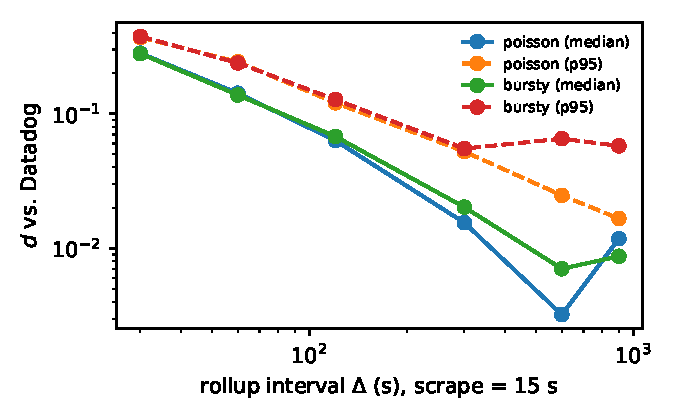
\includegraphics[width=0.6\linewidth]{figures/rate_error_vs_window}
\caption{Error of \texttt{rate()} against Datadog as the rollup interval grows, at a
$15$\,s scrape interval. \texttt{rate} is the only candidate whose error depends on the
data.}
\label{fig:rate-error}
\end{figure}

\subsubsection{The dual-write replay}
\label{sec:replay}

Everything to this point compares a PromQL candidate against our reading of Datadog's
rollup. That is a model, and a model is what \S\ref{sec:not-measured} warns the reader
about. This subsection closes the gap for the counter rules by running the dual-write
construction of this section literally: one stream of observations, written to both
systems, read back from both.

The stream is real. Counting the requests in a web-server access log into a scrape grid
gives a counter with the shape that \S\ref{sec:threats} says the synthetic workloads only
imitate: in the half hour used here the per-minute rate swings seventeenfold without
being asked to. We take the busiest half hour of the Kennedy Space Center HTTP logs of
July~1995~\citep{nasahttp}, count requests at a $15$\,s scrape interval into one counter
per HTTP status class, and write the cumulative series to Prometheus and its image under
$\phi_{\mathsf{zero}}$ --- the per-interval deltas --- to Datadog, at the same timestamps
(\texttt{scripts\slash replay\_dualwrite.py}).
The trace's publishers ask that it not be analysed beyond general traffic patterns, and
the parser enforces that rather than promising it: it keeps a timestamp and a status
class and discards the host and the request line, so what is replayed is a count of
requests per interval and nothing else. Timestamps are shifted to the present, because
Datadog's intake refuses points much older than an hour; the shape is real and the
absolute times are not.

\begin{table}[htbp]\centering\footnotesize
\begin{tabular}{@{}llrrr@{}}
\toprule
Scrape grid & PromQL candidate & Evaluated inside & On the edge & Max $d$ \\
\midrule
unaligned & \texttt{x - x offset $\Delta$} & 100.0\% & 100.0\% & 0 \\
 & \texttt{increase(x[$\Delta$] anchored)} & 100.0\% & 100.0\% & 0 \\
 & \texttt{rate(x[$\Delta$])} $\times\,\Delta$ & 20.2\% & 20.2\% & 1 \\
\addlinespace
aligned & \texttt{x - x offset $\Delta$} & 100.0\% & 27.4\% & 0 \\
 & \texttt{increase(x[$\Delta$] anchored)} & 100.0\% & 27.4\% & 0 \\
 & \texttt{rate(x[$\Delta$])} $\times\,\Delta$ & 20.2\% & 16.7\% & 1 \\
\addlinespace
\bottomrule
\end{tabular}

\caption{The dual-write replay: each candidate against \emph{Datadog}, bucket by bucket,
on a real request trace. ``Inside'' and ``on the edge'' are the two evaluation instants
of Remark~\ref{rem:closure}. $84$ comparisons per row.}
\label{tab:replay}
\end{table}

Table~\ref{tab:replay} is the result, and two things in it are worth separating.

The first is that both exact forms are exact --- against Datadog, not against a model of
it, on traffic nobody generated for the purpose. \texttt{rate} is not, at $20.2\%$ of
buckets on both grids, which is what \S\ref{sec:ingestion} has said throughout and what
the steady synthetic workload conceals by being steady. That figure used to read
$19$--$20\%$, a spread between the two grids that was not a property of either: the
replay script scored this one table by bit-identity where every other exactness column in
this paper uses a $10^{-12}$ relative bound, and one aligned bucket reading $236.0$
against $235.999\ldots$ counted as a disagreement.

The second is about the convention of Remark~\ref{rem:closure}, and it explains how that
convention came to be assumed wrongly for so long. On the unaligned grid --- a scrape
whose samples do not fall on rollup boundaries, which is what a jittered scrape produces
and therefore the ordinary case --- evaluating on the bucket's edge agrees with
evaluating inside it, on every bucket. Off a boundary the two half-open intervals contain
the same samples, so the closure is simply not observable. Snap the scrape grid onto the
rollup grid and the same comparison falls from $100\%$ to $27.4\%$. The error was
invisible in exactly the configuration real deployments have, and decisive in the one the
synthetic workloads of Table~\ref{tab:rollup-live} happen to use.

What this does not do is also worth stating. A request counter does not reset in half an
hour, so \texttt{COUNTER\_RESET} is not exercised here; the restart rows of
Table~\ref{tab:rollup-live} and the scripted reset of E1 (Remark~\ref{rem:rho}) are the
evidence for that case. It is one window of one
trace at one rollup interval. And it tests the counter rules, not translation coverage:
$\kappa$ is what it was.

\paragraph{What was assumed, and what is left.}
This section began with two facts about Datadog that its documentation does not settle,
and carried a third about its backend. None is still an assumption, and the two it began
with did not turn out the way they were guessed.

The reset policy $\rho$ is no longer among them either, and it is the one that was
settled twice: read from the agent's source and then put to a running agent, which
agreed with the reading (Remark~\ref{rem:rho}). It too went against the guess --- the
prediction recorded in advance was discarding the interval, which turns out not to be a
reset policy at all.

Bucket closure is no longer among them. Remark~\ref{rem:closure} settles it by
measurement: buckets are left-closed and named by their start, which is the opposite of
what an earlier draft of this section assumed and the opposite of PromQL's own
convention. Epoch alignment \emph{is} documented~\citep{ddrollup}, so the remaining
content of \texttt{ROLLUP\_ALIGNMENT} is sharper than ``align the grids'': a PromQL
window follows the evaluation step, and the step that reads a Datadog bucket is one
\emph{inside} its right edge rather than on it. Evaluating on the boundary --- the
obvious choice once the closure is known --- disagrees on every bucket where a scrape
lands on the boundary too, which is the ordinary case. The translator records
\texttt{ROLLUP\_ALIGNMENT} on every rollup it emits for that reason.

Nothing is left. The last of the three --- whether Datadog's backend stores what its
agent sends --- stood until a counter was made to reset on purpose, which is what the
replay above cannot do and what E1 does (Remark~\ref{rem:rho}). Both systems scrape one
endpoint across the reset; Datadog stores $103$ over the bucket holding it, and
\texttt{increase($x$[$60$s] anchored)} over Prometheus returns $103$ for the same bucket,
as it does on every complete bucket of all three counters. So the restart rows of
Table~\ref{tab:rollup-live} no longer stand alone: the anchored form tracks
$\phi_{\mathsf{zero}}$, and Datadog agrees with it where a counter actually restarts.


\section{Grammars (RQ1)}
\label{sec:grammars}
\todo{Core productions in Rich's notation; precedence encoding; LALR(1) construction
with no conflicts (from \texttt{qlport.parse}); conflicts met and resolved (e.g.\ keyword
prefixes such as \texttt{max\_over\_time}); Datadog grammar inference and corpus parse
rate (notebook 01).}

\section{Translation (RQ2)}
\label{sec:translation}
\todo{The IR and its denotations; syntax-directed lowering and emission; the gap
catalogue table (notebook 03).}

\subsection{Counter rollups}
The rules for \texttt{.as\_count()}, \texttt{.as\_rate()} and \texttt{.rollup(sum,
$\Delta$)} are established in Section~\ref{sec:ingestion}, where they belong: which
PromQL expressions may translate a Datadog rollup at all is a question about the
ingestion mapping, not about the emitter. Propositions~\ref{prop:offset}
and~\ref{prop:anchored} give the two exact forms and Table~\ref{tab:rollup-live} the
measurements. What the emitter adds is the choice between them and the preconditions it
reports: \texttt{COUNTER\_RESET} on the cumulative difference,
\texttt{ANCHORED\_VERSION} on the anchored form, and \texttt{ROLLUP\_ALIGNMENT} on
both.

\subsection{Where the rollup sits}
One structural fact about Datadog decides the shape of every translated query, and it is
easy to get backwards. A Datadog query is evaluated ``first by time, then by
space''~\citep{datadog}: the rollup reduces each series on its own, and the space
aggregator (\texttt{sum:}, \texttt{avg:}, \texttt{max:}, \texttt{min:},
\texttt{count:}, with its optional \texttt{by \{...\}}) then combines those reduced
values. PromQL's range functions have the same shape, so the translation is direct:
\begin{center}\footnotesize
\texttt{max:x\{*\}.rollup(avg, 60)}\quad$\longmapsto$\quad\texttt{max(avg\_over\_time(x[60s]))}
\end{center}

Nesting the two layers the other way round --- space aggregation first, rollup outside
--- describes a different query, and raises a question the real semantics never asks:
whether the two aggregators commute. They do for $(\mathsf{sum},\mathsf{sum})$,
$(\mathsf{max},\mathsf{max})$ and $(\mathsf{min},\mathsf{min})$, and not for
$\mathsf{max}$ or $\mathsf{count}$ over an averaging rollup, where PromQL would need a
subquery to put the rollup outside. An earlier version of this translator was built that
way and refused $348$ query occurrences --- four points of $\kappa$ --- on the strength
of that commutation argument. Every translation it \emph{did} emit was still correct,
because where the aggregators commute the two orders coincide, which is exactly what
makes the error hard to notice: the failure shows up only in the refusals.

% ---------------------------------------------------------------------------
% The regular sub-problem: Datadog glob <-> PromQL regex matcher.
% Numbers come from notebook 04 and data/processed/regex_glob.csv.
% ---------------------------------------------------------------------------

\section{The Regular Sub-problem}
\label{sec:regular}

Both languages filter on tag values, and both do it with a pattern language, but not the
same one. Datadog's is a glob; PromQL's is a regular expression. One is a proper subclass
of the other, so the two directions of this sub-problem are not the same question asked
twice: the main direction needs a translation that always exists, and the reverse
direction needs a decision procedure for whether one does. This section gives both, and
the decision procedure is where the course's machinery does the work.

\subsection{Globs, and what they can say}
\label{sec:globs}

\begin{definition}[Tag glob]\label{def:glob}
Fix an alphabet $\Sigma$ of tag-value characters. A \emph{glob} is a string over
$\Sigma\cup\{*\}$, written $g=s_0*s_1*\cdots*s_n$ with $n\ge 0$ stars and literal
segments $s_i\in\Sigma^{*}$. It denotes
\[
L(g)=\{\,s_0w_1s_1w_2\cdots w_ns_n \;:\; w_i\in\Sigma^{*}\,\}.
\]
Datadog documents prefix, suffix and substring wildcards and no other
construct~\citep{ddfilter}: there is no single-character wildcard, no alternation inside
a value, no character class, and no escape that would make a literal
\texttt{*}. Write $m(g)=\sum_i|s_i|$ for the total literal length.
\end{definition}

The main direction needs only the easy half, and gets it by construction.

\begin{proposition}[Globs are regular, uniformly]\label{prop:glob-regex}
Let $\mathrm{glob}(g)$ be the regular expression obtained from $g$ by replacing every
\texttt{*} with \texttt{.*} and escaping every other character. Then
$L(\mathrm{glob}(g))=L(g)$, where the regular expression is read under PromQL's whole-value
anchoring.
\end{proposition}
\begin{proof}
Induction on $n$. For $n=0$ both sides are $\{s_0\}$. For the step, \texttt{.*} denotes
$\Sigma^{*}$ and concatenation of regular expressions denotes concatenation of languages,
which is exactly how Definition~\ref{def:glob} quantifies $w_i$. Anchoring matters: it is
what makes the outermost concatenation span the whole value, and it is the fact
Proposition~\ref{prop:disjunction} rests on, read off a real server there rather than
assumed.
\end{proof}

\noindent
Every glob therefore has an exact PromQL matcher, which is why no gap code in
Section~\ref{sec:gaps} mentions globs on tag \emph{values}. The remaining direction is
the interesting one, and one structural fact decides most of it.

\begin{lemma}[Dichotomy]\label{lem:dichotomy}
For every glob $g$: if $n=0$ then $L(g)=\{s_0\}$ is a single word; and if $n\ge 1$ then
$L(g)$ contains a word of every length $\ell\ge m(g)$, and every word of $L(g)$ contains
each $s_i$ as a factor, in order.
\end{lemma}
\begin{proof}
The first case is immediate. For the second, taking $w_1\in\Sigma^{\ell-m(g)}$ and
$w_i=\varepsilon$ for $i>1$ gives a word of length $\ell$; the factor claim is
Definition~\ref{def:glob} read left to right.
\end{proof}

\noindent
So a glob language is either a singleton or unbounded in length. That is a strong
restriction, and it settles each construct the corpus refuses --- not by measurement but
by proof.

\begin{corollary}[Three things no glob says]\label{cor:no-glob}
Assume $|\Sigma|\ge 2$. Then
\begin{enumerate}
\item no glob denotes a finite language with two or more words --- in particular none
denotes $\Sigma$, so there is no single-character wildcard, and none denotes an
alternation of distinct literals;
\item no glob denotes $\Sigma^{+}$, the non-empty values;
\item for $\emptyset\neq A\subsetneq\Sigma$, no glob denotes $A^{+}$ --- a star cannot be
restricted to part of the alphabet.
\end{enumerate}
\end{corollary}
\begin{proof}
(1) A finite language with two words is neither a singleton nor unbounded, so
Lemma~\ref{lem:dichotomy} excludes it. (2) $\varepsilon\notin\Sigma^{+}$ forces
$m(g)\ge 1$, since $m(g)=0$ makes $g$ a string of stars and $\varepsilon\in L(g)$; and
$\Sigma^{+}$ contains words of length $1$, so $m(g)\le 1$. Hence $m(g)=1$: $g$ has a
single literal character $c$ and at least one star. By Lemma~\ref{lem:dichotomy} every
word of $L(g)$ contains $c$, while $\Sigma^{+}$ contains the one-character words of
$\Sigma\setminus\{c\}$, which is non-empty. (3) The same argument gives $m(g)=1$ with one
literal $c$, which must lie in $A$ since every word of $L(g)$ contains it. A single
literal and at least one star leaves three shapes: $c{*}$, ${*}c$ and ${*}c{*}$. In the
first and third $L(g)$ contains $c\sigma$ for every $\sigma\in\Sigma$; in the second it
contains $\sigma c$ for every $\sigma$. Either way it contains a word using a
$\sigma\notin A$, which $A^{+}$ does not, and $\Sigma\setminus A\neq\emptyset$.

Taking $c\sigma$ in every case, as an earlier version of this proof did, is wrong for
$g={*}c$: that language has no word beginning with $c$ unless $c$ repeats.
\end{proof}

\subsection{Deciding whether a regex has a glob}
\label{sec:decide}

Corollary~\ref{cor:no-glob} rules particular shapes out. The general question --- given a
regular expression, is there \emph{any} glob denoting the same language? --- is settled by
a single observation about shortest words.

\begin{proposition}[Glob-expressibility is decidable]\label{prop:decidable}
Let $r$ be a regular expression with $L(r)\neq\emptyset$, and read \texttt{*} as matching
the empty string. It is decidable whether some glob $g$ has $L(g)=L(r)$, and a witness is
produced when one exists.
\end{proposition}
\begin{proof}
Suppose $L(r)=L(g)$ for $g=s_0*\cdots*s_n$. Taking every $w_i=\varepsilon$ gives the word
$s_0s_1\cdots s_n\in L(g)$ of length $m(g)$, and every other word of $L(g)$ has some
$w_i\neq\varepsilon$ and so is strictly longer. Hence $s_0s_1\cdots s_n$ is the shortest
word of $L(g)$ \emph{and the only word of that length}.

So the procedure is: construct a DFA for $r$ --- Rich's regular-expression-to-FSM
construction (Thm 6.1) followed by the subset construction (Thm 5.3) --- and find its
shortest accepted
word $w$ by breadth-first search from the start state, together with the number of
accepting paths of that length. If $L(r)$ has no unique shortest word, no glob exists. If
it does, then $w=s_0s_1\cdots s_n$, so $g$ is $w$ with stars inserted at some subset of
its $|w|+1$ gaps: at most $2^{|w|+1}$ candidates. Each is settled by deciding
$L(r)=L(\mathrm{glob}(g))$, which is decidable by Rich Thm 9.5. The search is finite and
exhaustive, so it answers either way.
\end{proof}

\noindent
Two remarks on making this run. Breadth-first search is not an optimisation but the
method: enumerating candidate words in order instead, as a general-purpose regular-language
library does, does not terminate in practice on a corpus regex whose shortest word is
sixty characters over a twenty-character alphabet. And the $2^{|w|+1}$ candidates can be
pruned without losing completeness, because inserting stars only grows the language: any
star belonging to a solution must, on its own, keep the candidate inside $L(r)$, so gaps
failing that single subset test cannot appear in any solution at all. On the corpus this
leaves a handful of candidates rather than $2^{61}$.

\subsection{Unions, and the same fact in both directions}
\label{sec:glob-unions}

A single glob is the wrong target. A Datadog scope can disjoin over one tag key, as
$k \in (g_1,\dots,g_B)$ or as $k{:}g_1 \vee \cdots \vee k{:}g_B$, and
Proposition~\ref{prop:disjunction} showed that such a scope is exactly one PromQL
alternation matcher. Read in this direction the same proposition says that the reverse
translation of a regular expression should be sought as a \emph{finite union} of globs,
and $\mathtt{LIST|GET}\mapsto k \in (\texttt{LIST},\texttt{GET})$ is then immediate. The
two directions are not two results; they are one fact used twice.

The union must be bounded, and the bound is part of the claim rather than an
implementation detail. Every finite language is a union of singleton globs, one per word,
so boundedness is what stops the question from being trivial --- and it is not only a
matter of taste. By Corollary~\ref{cor:no-glob} no glob denotes $\Sigma^{+}$, yet
$\bigcup_{c\in\Sigma}L(c*)=\Sigma^{+}$, so the non-empty values \emph{are} a finite union
of globs: one for every character of the alphabet. A scope is a piece of text somebody
maintains, so a union of a million branches is not a translation. We fix $B=64$ and
report anything needing more as a refusal, naming the bound.

Whether glob-union-expressibility is decidable without a bound we leave open. The shortest-word
argument does not transfer: each glob of a minimal union contributes its own shortest
word, and nothing bounds those by the shortest word of the union, so the candidate space
is no longer finite. Within the bound the procedure used here is sound but not known to be
complete --- it proposes a union from the regular expression's syntax and then decides
equivalence, so what it returns is exact, while a refusal is in general a statement about
the proposer. Proposition~\ref{prop:decidable} removes that caveat for the single-glob
case, and Section~\ref{sec:glob-corpus} uses it to check the refusals rather than trust
them.

\subsection{What the corpus contains}
\label{sec:glob-corpus}

\begin{table}[htbp]\centering\footnotesize
\begin{tabular}{@{}lrrrr@{}}
\toprule
Outcome & Distinct & Share & Occurrences & Share \\
\midrule
One glob & 61 & 33.2\% & 309 & 29.7\% \\
A finite union of globs & 73 & 39.7\% & 344 & 33.0\% \\
Neither ($\bot$) & 50 & 27.2\% & 388 & 37.3\% \\
\emph{Template-valued, not a regex} & 174 & --- & 7,546 & --- \\
\bottomrule
\end{tabular}

\caption{Every \texttt{=\textasciitilde{}} and \texttt{!\textasciitilde{}} matcher in the
PromQL half of the corpus. Shares are of the concrete regular expressions; the
template-valued row is counted but not classified, because the pattern is not in the query
text.}
\label{tab:regex-glob}
\end{table}

The first result is not about regular languages. Of $8{,}587$ regex matchers,
$7{,}546$ --- $87.9\%$ --- have a Grafana template variable as their pattern, as in
\texttt{\{pod=\textasciitilde{}"\$pod"\}}. The value is chosen when somebody looks at the
dashboard, so there is no pattern to convert; the normalisation of
Section~\ref{sec:corpus} deliberately leaves these alone, because the matcher already
parses with the variable in place. For these the reverse direction is not hard but
\emph{statically undefined}, and that is a property of how dashboards are written rather
than of either language.

Among the $1{,}041$ occurrences whose pattern is concrete, Table~\ref{tab:regex-glob}
gives the three-way split and Table~\ref{tab:regex-glob-examples} what each outcome
looks like. A glob exists for $653$ of them ($62.7\%$), but for more than
half of those only as a union: one glob covers $309$ occurrences ($29.7\%$) and a bounded
union covers $344$ ($33.0\%$). Those counts rose in the seventh reading of the apparatus,
and the caption of Table~\ref{tab:regex-glob} is why: it says ``every \texttt{=\textasciitilde{}}
and \texttt{!\textasciitilde{}} matcher'', and the scanner behind it accepted only
double-quoted patterns. PromQL writes a string three ways, its own grammar in
Section~\ref{sec:grammars} says so, and $114$ matcher occurrences sat in the other two. Treating a single glob as the target --- the obvious
reading of ``does this regex have a glob'' --- would therefore have understated the
reverse direction by $33.0$ points of occurrence coverage, and the construction that
recovers them is the one Section~\ref{sec:translation} already proved for the other
direction.

\begin{table}[htbp]\centering\footnotesize
\begin{tabular}{@{}lrrl@{}}
\toprule
Construct with no glob & Distinct & Occurrences & Shortest example \\
\midrule
No non-empty wildcard (\texttt{.+}) & 21 & 238 & \texttt{.+} \\
No single-character wildcard (\texttt{.}, \texttt{5..}) & 26 & 140 & \texttt{5..} \\
No bounded alphabet under a star (\texttt{[a-z]+}) & 3 & 10 & \texttt{5[0-9]+} \\
\bottomrule
\end{tabular}

\caption{The constructs behind the $388$ refused occurrences. Each is ruled out as a
single glob by Corollary~\ref{cor:no-glob}; only the third is also beyond a bounded
union of them.}
\label{tab:regex-glob-reasons}
\end{table}

\begin{table}[htbp]\centering\footnotesize
\begin{tabular}{@{}llr@{}}
\toprule
PromQL regex & Datadog scope value & Occurrences \\
\midrule
\texttt{\textasciicircum{}k8s\_.*} & \texttt{k8s\_*} & 60 \\
\texttt{.*external-dns.*} & \texttt{*external-dns*} & 36 \\
\texttt{.*pod.*} & \texttt{*pod*} & 24 \\
\texttt{LIST|GET} & \texttt{GET, LIST} & 41 \\
\texttt{ext.*|xfs} & \texttt{ext*, xfs} & 34 \\
\texttt{proxy|attach|log|exec|portforward} & \texttt{attach, exec, log, portforward, p\dots{}} & 32 \\
\texttt{.+} & $\bot$ No non-empty wildcard & 133 \\
\texttt{(/dev/)?(mmcblk.p.+|nvme.+|rbd.+|\dots{}} & $\bot$ No non-empty wildcard & 49 \\
\texttt{5..} & $\bot$ No single-character wildcard & 40 \\
\bottomrule
\end{tabular}

\caption{The three most frequent regular expressions of each outcome.}
\label{tab:regex-glob-examples}
\end{table}

Table~\ref{tab:regex-glob-reasons} is the part this section can be held to, and it has
to be read against the target of \S\ref{sec:glob-unions} rather than against a single
glob. Three constructs account for every refusal, and each is an instance of
Corollary~\ref{cor:no-glob} \emph{or} of one of the two facts below: a single-character
wildcard such as \texttt{5..} would need a
glob for $\Sigma$, which part~(1) forbids; \texttt{.+} would need one for $\Sigma^{+}$,
forbidden by part~(2); and \texttt{5[0-9]+} would need a star confined to the digits,
forbidden by part~(3).

``Each is an instance'' is the part that needed care, and an earlier version of this
sentence overstated it. The corollary is about three \emph{specific} languages and is
closed under neither concatenation with a literal nor union, while most refused corpus
patterns are of those shapes: \texttt{dm-.+} is not $\Sigma^{+}$, and
\texttt{5[0-9]+} is not $A^{+}$, because $A^{+}$ contains words of length one and that
language's shortest word has three characters. Two facts close the gap, and both are
already in this section rather than new.

The first is the uniqueness step inside Proposition~\ref{prop:decidable}'s proof: if
$L(r)=L(g)$ then $L(r)$ has a \emph{unique} shortest word. Most of the patterns the
corollary does not reach fail that immediately --- \texttt{dm-.+} has shortest words
\texttt{dm-} and nothing else of that length only if the suffix can be empty, which
\texttt{.+} forbids, so its shortest words are \texttt{dm-}$\sigma$ for every $\sigma$,
and there are $|\Sigma|$ of them. The second is the generalisation part~(3) is an
instance of: \emph{if $L$ is infinite and some $\sigma\in\Sigma$ occurs in no word of
$L$, then $L$ is no union of finitely many globs}, because an infinite glob language
needs a star and a star admits every character. That is what the prose below has always
said, and stating it as a fact rather than as an aside is what the $10$ unconditional
occurrences actually rest on.

The three are not equally final, and saying so costs less than leaving it implied. The
target here is a union of at most $B$ globs, and the first two constructs \emph{are}
finite unions: $\Sigma^{+}$ is $\bigcup_{c\in\Sigma}L(c*)$ and $\Sigma$ is the union of
its one-character words, so each needs one branch per alphabet character, or
$|\Sigma|^{2}$ of them for \texttt{5..}. Those refusals therefore rest on the bound as
well as on the corollary, and on an alphabet larger than $B$, which this paper does not
pin down --- the proposer refuses them structurally rather than by counting branches.
Only part~(3) is unconditional: an infinite language needs a star, a glob's star admits
every character, and no union of finitely many such globs confines it to the digits. So
$378$ of the $388$ occurrences are refused by a theorem about single globs plus a bound
this paper chose, and $10$ by a theorem about globs outright. For
the single-glob question we can also say it the other way round, by measurement rather
than by proof: re-deciding every concrete regular expression with the complete procedure
of Proposition~\ref{prop:decidable} reaches \emph{all} $184$ distinct patterns --- the
counts in this paragraph are of patterns rather than of the occurrences above --- and
disagrees with the syntax-directed proposer on \emph{none} of them. It recovers the
same glob for all $61$ of the single-glob cases, and finds no glob for all $50$ refusals
and all $73$ unions. Nothing is left undecided: no pattern exceeds the search's own
candidate bound, so the agreement is over the whole population rather than over a
reachable part of it.

An earlier version of this paragraph reported $168$ of $183$ and recorded the remainder
as not reached, which was a statement about a clock rather than about the procedure. The
script takes a time budget, that run was given $2{,}400$\,s, and four patterns of one
family --- a parenthesised alternation inside a long literal, as in
\texttt{cnpg\_pg\_stat\_(bgwriter|checkpointer)\_checkpoints\_timed} --- cost $91$ to
$176$ seconds each when timed on an idle machine, so the budget expired partway through
them. Run without one the cross-check takes $4{,}725$\,s and finishes. What makes those
patterns expensive is worth naming, because it is the procedure working rather than
struggling: the shortest word of such a pattern is forty-odd characters, so the pruned
space of star insertions is large, and the search has to \emph{exhaust} it to conclude
that no single glob exists. The costly cases are the negative ones, and they are exactly
the cases a structural proposer's refusal would otherwise have to be taken on trust. The run is cached
(\texttt{scripts\slash crosscheck\_globs.py}), and \texttt{tests\slash test\_regular.py}
fails if a disagreement ever appears, if any pattern goes unreached, or if the two sides
stop sharing a population.

One qualification on ``complete''. The search is complete for the regular expressions its
parser accepts, which is the dialect of the equivalence library rather than all of
PromQL's: a pattern carrying an interior anchor, or one whose escapes the structural
proposer normalises first, is refused by the search where the proposer answers. No corpus
pattern is of either shape --- all $184$ were reached --- so the agreement reported above
is over the whole population, but the word means complete relative to that dialect.

\begin{remark}[The largest refusal turned on an undocumented detail]%
\label{rem:star-empty}
$238$ of the $388$ refused occurrences are \texttt{.+} or a pattern containing it,
including the corpus's most common concrete regular expression (\texttt{.+}, $133$
occurrences) and its most elaborate one
(\texttt{(/dev/)?(mmcblk.p.+|nvme.+|\dots{})}, $49$). They are refused by
Corollary~\ref{cor:no-glob}(2) --- but that part of the corollary assumed \texttt{*}
matches the empty string, and Datadog does not document whether it does. The two readings
cannot both be wrong and cannot both be right: a glob has exactly one wildcard, which
either requires a character or does not, so under one reading \texttt{.+} has no glob and
under the other \texttt{.*} has none. The corpus uses \texttt{.+} $133$ times and
\texttt{.*} $9$ times, so the reading is worth $124$ occurrences either way.

It is settled, and in favour of the reading taken here. Submitting two series of one
metric whose \texttt{probe} tag is \texttt{web-} and \texttt{web-1}, and filtering on
\texttt{probe:web-*}, returns both: the wildcard matches the empty string. So
\texttt{.*} has a glob, \texttt{.+} has none, and the figures above stand as computed
(\texttt{scripts\slash trial\_checks.py e5}, cached and regression-tested).
\texttt{regular.py} still records the reading in a single constant, so the measurement
can be redone under the other one if Datadog's behaviour changes.
\end{remark}

\noindent
The practical conclusion for the reverse direction is narrower than
Table~\ref{tab:regex-glob} suggests on its own. A Datadog scope cannot say what
\texttt{5..} says, and cannot say what \texttt{.+} says under the reading taken here, in
any scope a person would maintain; both are ordinary things to write in PromQL. That is
the kind of gap this paper set out to distinguish from the other kind, and in this
corner of the problem no refusal is unfinished work: each is either a theorem about
globs or that theorem together with the branch bound, and neither is removed by
building more.

\section{Evaluation (RQ3)}
\label{sec:evaluation}
\todo{Pipeline (state it: e.g.\ OpenTelemetry exporting to both systems); dual-write
harness; corpus; empirical checks of Datadog's reset policy and bucket boundaries;
$\kappa$ overall and by gap; untested queries reported separately (notebook 05).}

\section{Discussion}
\label{sec:discussion}
\todo{Is the lock-in syntactic or semantic? \S\ref{sec:gaps} answers this for the main
direction and the answer is mostly ``neither'': $2.4\%$ of the corpus is unimplemented
work against $2.0\%$ that PromQL cannot express, so going this way the switching cost is
engineering. The language-design argument therefore rests on the reverse direction and on
the staircase, and \S\ref{sec:regular} is now the concrete evidence for the first:
there the refusals are \emph{all} of the expressiveness kind, each one a corollary of the
glob dichotomy rather than unfinished work, and they cover $38.3\%$ of the concrete
patterns. Contrast that proportion with the gap catalogue's and say what the asymmetry
means --- going to Prometheus costs engineering, coming back costs expressiveness.
Direction asymmetry: proved as Remark~\ref{rem:directional}, so discuss what it means
rather than restating it. The staircase of \S\ref{sec:staircase} as a switching cost in
its own right. The $88.0\%$ of matchers that are template variables
(\S\ref{sec:glob-corpus}) belong here too: a portability claim about dashboards is partly
a claim about a templating layer neither query language contains. LogQL and SPL.
Threats specific to the discussion (\S\ref{sec:threats} has the empirical ones):
synthetic workloads for the rollup measurements, and the Datadog facts of
\S\ref{sec:not-measured} that no experiment here settles --- bucket closure, and the
reading of \texttt{*} that Remark~\ref{rem:star-empty} turns on. Do \emph{not} list
\texttt{anchored} as modelled --- it is verified against Prometheus~3.15.0 in
Table~\ref{tab:model-verification}.}

% ---------------------------------------------------------------------------
% Answers the four questions, separates what is established from what is
% assumed, and says what the next measurement would be.
% ---------------------------------------------------------------------------

\section{Conclusion}
\label{sec:conclusion}

\paragraph{The four questions.}
\textbf{RQ1.} Both languages admit deterministic one-token-lookahead parsers, with an
asymmetry that is itself a finding. The inferred Datadog grammar --- the first published
grammar for that language --- is conflict-free. PromQL has $2$ shift/reduce conflicts,
both on the parenthesis that begins either a vector-matching label list or a parenthesised
operand, and both forced by that list's optionality rather than by how we layered the
rules; so RQ1's answer for PromQL is ``LALR(1) modulo one documented resolution'', for
this grammar, with no claim that none does better. Neither answer is where the switching
cost lives, which is itself worth knowing.

\textbf{RQ2.} The largest exactly-translating fragment we could build covers $96.3\%$ of
Datadog query occurrences, and the soundness theorems of \S\ref{sec:kernel-soundness} and
\S\ref{sec:binop-soundness} between them cover every expression the translator emits, so
nothing is shipped that is not proved. Outside the fragment, $1.2\%$ of the corpus is
beyond reach --- four constructs, two of them information barriers rather than
expressiveness gaps --- against $2.4\%$ that is work this translator has not done, a
ceiling of $98.7\%$. In the reverse direction, on the sub-problem of tag filtering, the
obstructions are theorems: a glob's language is a single word or unbounded in length, and
three impossibility results follow. With a stated bound on union size they account for
every refusal we measure --- $37.3\%$ of the matcher occurrences whose pattern is
concrete --- and $10$ of those need no bound at all.

\textbf{RQ3.} Coverage on published dashboards is the $96.3\%$ above, and the shape of
the shortfall matters more than its size: coverage against implementation effort is a
staircase rather than a curve, because a query translates only when every feature it uses
is supported, while the popularity that would guide an implementation order is marginal.
Half the work does not port half the estate.

\textbf{RQ4.} No. A dashboard query does not determine its own meaning, and this is the
answer we would now put first. Of the translations we emit, $96.9\%$ depend on a rollup
interval the source query leaves to the dashboard's time range, and $100\%$ on a metric
type no query in either language declares. Neither is a defect of one vendor: $88.6\%$ of
Datadog query occurrences and $82.5\%$ of PromQL ones carry at least one template
variable, so in both languages the object a migration ports is a schema plus a
resolution layer that belongs to the dashboard tool. One of the two assumptions is
checkable, because the repository the dashboards come from declares each metric's type,
and where it can be checked our inference is wrong for $6.5\%$ --- $491$ occurrences,
more than the whole inexpressible column. $\kappa$ counts those as translations.
Coverage and correctness differ, by a measured amount, and no coverage number could have
told us: a query that does not fix its own meaning parses and translates like any
other.

\noindent
What each of those answers rests on --- what is proved, what is verified against a real
server, what is measured against the vendor, and what is still assumed --- is set out
\apref{app:experiments}. Three of the eight vendor measurements contradicted what this
paper had assumed before asking.

\iffull% The inventory of evidence that closed the conclusion: proved, verified against a
% real server, read and written down, measured against the vendor, and assumed.
\subsection{What rests on what}
\label{app:evidence}

Three things in this paper are proved: the directional information barrier, whose
reverse half is Proposition~\ref{prop:reverse} and holds for every possible translator
and not only ours; the exactness of the rollup translations on a
stated class, with the preconditions enumerated as the hypotheses of a theorem; and the
non-expressibility results of \S\ref{sec:regular}. Three things are verified against a
real Prometheus~3.15.0 rather than a model, with the responses cached and
regression-tested: the PromQL semantics the rollup rules depend on, the anchoring of
label-matcher regular expressions, and the series pairing that
Theorem~\ref{thm:arith} rests on. Two further readings were taken from a real server
and written down as prose rather than cached --- the parse error that decides
\S\ref{sec:grammars}'s two conflicts, and the rejection that
Remark~\ref{rem:anchored-flag} turns on --- so they are evidence of a weaker kind than
the three above, and the difference is in the artefact rather than in the reading.
Nothing is left that was read from source and not then measured: Datadog's reset policy was taken from its
open-source agent at a pinned commit and afterwards put to a running one.

Eight things are measured against the vendor itself rather than assumed: the bucket
convention (left-closed and named by its start, the opposite of what this work assumed
until it asked), the automatic rollup interval as a function of the query range, the
default time aggregator of a bare query on a counter, whether a glob's \texttt{*} matches
the empty string, where \texttt{.as\_rate()} sits relative to the rollup and to the space
aggregation, what \texttt{.weighted()} computes, what \texttt{top(...)} ranks by and over
which window, and the reset policy --- read first from
the agent's source and then put to a running agent, which agreed with the reading. Five
of the eight confirmed what the paper had assumed. Three did not: the bucket convention;
\texttt{.as\_rate()}, which turned out to divide the aggregated result rather than
each series, and whose presence in a query turned out not to establish the metric's type
at all, because Datadog accepts the modifier on a gauge and ignores it; and
\texttt{.weighted()}, carried here as the largest single entry in the inexpressible
column until the account was asked and returned the same number with the modifier and without it. The last of the
eight decides which column $139$ corpus occurrences belong in, and is the only one
measured on both sides: over one workload, the candidate expression against a real
Prometheus in $20$ cases and \texttt{top()} itself against Datadog in $22$, each
agreeing with the documented rule throughout.

One assumption is settled from the vendor's source tree rather than from its API, and
it is the one that held of all the output. Every translation carries
\texttt{METRIC\_TYPE\_UNKNOWN} because a dashboard does not record whether a metric is
a counter or a gauge --- but \texttt{integrations-core} declares the type of each
metric it ships, in a file beside the dashboards that the corpus fetch had passed over.
For the $89.5\%$ of translated occurrences whose metric is declared, the front end's
inference is wrong on $6.5\%$: $491$ occurrences against the $0.8\%$ this
paper calls beyond reach (Remark~\ref{rem:type-measured}). $\kappa$ counts them as
translations, so the gap between coverage and correctness has a number for the first
time, and it is not zero.

One thing that was assumed throughout is now measured. The counter rules are checked
against Datadog itself, by replaying a real request trace into both systems and comparing
bucket by bucket (\S\ref{sec:replay}): both exact forms are exact and \texttt{rate} is
not. The one part a replay cannot reach is the reset policy, because a request counter
does not restart in half an hour; that took a counter built to restart, scraped across
the reset by a real agent and a real Prometheus at once, and it is the last assumption of
\S\ref{sec:ingestion} to be retired (Remark~\ref{rem:rho}).

The same construction has since been run at corpus scale, and it is the reason $\kappa$
can now be read as a statement about translations that were checked rather than merely
emitted. Abstracting the identifiers away --- and nothing a query would emit differently ---
collapses the corpus to $332$
distinct query shapes, few enough that a single trial account holds every series they
need; each is instantiated, written to both systems and compared bucket by bucket
(\S\ref{sec:differential}). It found four translation defects that the unit tests and the
single-trace replay had both missed --- and, six times over, found its own harness
first, which is the more useful lesson about differential rigs than the agreement rate
is.
\fi

\paragraph{What we would do next.}
The reverse translator: \S\ref{sec:regular} suggests the interesting results are there, and a
$\kappa$ for that direction would turn this paper's asymmetry claim from an argument into
a measurement. Further out, the method is language-agnostic wherever a language denotes a
function of a database at an instant, which brings LogQL within reach and leaves SPL
outside it.

\paragraph{The answer.}
Is the switching cost a language-design artefact? Partly, and not where we expected. In
the direction teams travel it is mostly engineering --- a finding this paper four times
nearly got wrong in the more quotable direction, through a structural error in the
translator, a rule it had not implemented, a modifier it never asked the vendor about,
and a classification that contradicted its own text. The artefact in that direction is
subtler than an expressiveness gap and is not a property of either language on its own: a
dashboard query does not say what it means, so every translation we emit is exact only
relative to context that arrives from the layer above both languages. The expressiveness
gap is real, provable, and in the direction teams do not travel.

That is the asymmetry --- leaving costs work, returning costs something work cannot buy
--- and it is worth being exact about whom it binds, because it is not the mechanism the
lock-in literature usually describes. We measured the exit and found it cheap. What is
expensive is the return, so nobody is held by what we measured; a team that wants to
leave, can. The cost falls instead on the team that has left and wants back, and on the
team that will not leave because it cannot price the option to return. That is a cost of
irreversibility rather than of captivity, and it is paid by a different decision at a
different time. Our two directions are also drawn from different populations ---
$\kappa$ over whole queries against a share of concrete tag-filter patterns, with no
reverse translator built --- so the asymmetry is an argument from two measurements and
not yet one measurement of two directions. Making it the latter is the next thing to do.



% --- apparatus -----------------------------------------------------------------
% In the full build each of these is \input inline by the section it belongs to, so it
% reads in place. In the deferred build the sections omit them and they land here as
% appendices instead. One copy of the prose either way: the two builds cannot drift,
% which after two passes of tables outrunning the text they quote is not a theoretical
% concern, with one class of exception. Where moving a block would leave a body statement
% with no support at all in the short build, the body carries a paragraph summarising the
% apparatus, which in the complete build reads as a signpost to the material below it.
% Those are the only prose in the paper that exists as a summary of other prose. Their
% figures are bound in tests/test_paper_figures.py, so a summary cannot drift from what it
% summarises even though the sentences are not the same sentences.
\iffull\else
\appendix
\apphead{Proofs and constructions}{app:proofs}

The statements these discharge are in the body, each at the point where it is used. In the
complete build they appear there too; here they are collected because a twenty-page
submission is read for its results and a proof is read when a result is doubted.

\begin{proof}
Since $\phi_\rho(D)=\phi_\rho(D')$, the source query receives the same input in both
cases:
\[
r:=\sem{q}_{\mathrm{DD}}(\phi_\rho(D),t)=\sem{q}_{\mathrm{DD}}(\phi_\rho(D'),t).
\]
Soundness would give $d(r,\sem{p}_{\mathrm{PQ}}(D,t))\le\varepsilon$ and
$d(r,\sem{p}_{\mathrm{PQ}}(D',t))\le\varepsilon$. Because $d$ is a metric on results with
matching label sets (and $\infty$ otherwise), the triangle inequality yields
\[
d\big(\sem{p}_{\mathrm{PQ}}(D,t),\sem{p}_{\mathrm{PQ}}(D',t)\big)\le 2\varepsilon . \qedhere
\]
\end{proof}

\begin{proof}[Proof of Proposition~\ref{prop:quantile}]
Let $[a,c)$ be a bucket of $B$ of positive width, which exists whenever $|B|\ge2$; for
$|B|\le1$ take a bucket of infinite width, of which there is always one, and work inside
it. Put $m=(a+c)/2$, let $0<r<(c-a)/2$ so that $m\pm(n-1)r$ stays inside the bucket for
the $n$ fixed next, and take
\[
n = 2+\Big\lceil \tfrac{1}{\min(p,\,1-p)} \Big\rceil .
\]
For $p\le\tfrac12$ let $X$ be $m-(n-1)r$ together with $n-1$ copies of $m+r$; for
$p>\tfrac12$ let $X$ be $n-1$ copies of $m-r$ together with $m+(n-1)r$. In both cases let
$Y$ be $n$ copies of $m$.

Every observation of either multiset lies in the chosen bucket, so the $B$-bucket counts
agree at $n$ there and $0$ elsewhere. The sums agree: in the first case
$m-(n-1)r+(n-1)(m+r)=nm$, in the second $(n-1)(m-r)+m+(n-1)r=nm$, and $Y$ sums to $nm$.
The counts agree at $n$. And $q_p(Y)=m$ under either convention, while $n$ is large
enough that the position $p$ selects in $X$ falls strictly inside the run of $n-1$ equal
observations --- so $q_p(X)=m+r$ in the first case and $m-r$ in the second, under
nearest-rank and under linear interpolation alike. Hence $q_p(X)\neq q_p(Y)$.

Two things about this are corrections rather than presentation. The witness was
$X=\{m-r,m+r\}$ against $Y=\{m,m\}$ for fifteen passes, separated ``under any convention
that returns an observed value'' --- a hedge that restricted the proposition and not
merely the proof, since under linear interpolation $q_{1/2}(X)=m=q_{1/2}(Y)$ and the
witness fails at exactly the quantile a reader would try first. The construction above
needs no hedge. And the proof computed medians while the statement quantifies over all
$0<p<1$, which the choice of $n$ now answers; the $|B|\le1$ branch said ``any two
distinct positive observations'', which may straddle the single boundary and so need not
share a bucket at all.

A third thing is not a correction but is worth keeping. The witness is chosen to survive
more than the bucket counts, which is what the corollary below needs and what an earlier
version did not supply. It took $X$ to be $n$ copies of $a$ against $n$ copies of
$(a+c)/2$: those agree on bucket counts and differ in their \emph{sum}, so
\texttt{histogram\_sum} separates them and they witness nothing about expressions over
everything Prometheus stores.
\end{proof}


\inlineonly{\noindent}%
The witness behind Corollary~\ref{cor:rate} is small enough to state, and it is worth
stating because it is a fact about Prometheus rather than about $\phi$. Four samples
$15$\,s apart inside a $60$\,s window, rising by $10$ each time, so $\phi_\rho$ is three
deltas of $10$ wherever the counter starts and no series begins inside the window. At a
first value of $1$ the \texttt{durationToZero} clip binds and the start-of-window
extrapolation is cut to $1.5$\,s; at $4$ it does not bind and the full $5$\,s to the
window edge is used. The readings are $0.628$ and $0.667$ --- and the dependence is
confirmed against a real Prometheus~3.15.0 rather than against this paper's model of it.

\noindent
Two earlier versions of the corollary were wrong about this, and the second way is the
one worth recording. The first claimed that on $\mathcal{C}_{\mathrm{warm}}$ ``the
remaining inputs to the extrapolation --- the increase over the window and the sample
spacing --- all survive $\phi_\rho$''. They do not exhaust the inputs, which is what the
witness above shows. The second was this appendix: the witness was measured, written up
here, and the conclusion drawn correctly --- and the corollary three lines above it went
on asserting invariance on $\mathcal{C}_{\mathrm{warm}}$ for eleven further passes, so
the paper stated a claim and its refutation on facing pages. That is the failure mode
\S\ref{sec:discussion} catalogues, found in this paper's own prose rather than in its
instruments: a correction is only made where it is carried to everything that rests on
it. Nothing else rested on this one --- \S\ref{sec:translation} cites
Corollary~\ref{cor:raw}, not this one, and \texttt{rate} is never emitted --- which is
why it survived so long.

\noindent
Corollary~\ref{cor:rate} is worth stating carefully, because it marks the limit of what
invariance buys. Invariance is \emph{necessary} for a sound translation and not
sufficient, and \texttt{rate} fails both: it is inadmissible wherever the extrapolation
reads an absolute value, and even where it is admissible it is not exact, since
extrapolating to the window edges computes a different quantity from the bucket sum
Datadog reports. Admissibility rules candidates out; exactness has to be established
separately.

\begin{proof}
An instant selector at $u$ returns $v_{\ell(u)}$ for $\ell(u)=\max\{i:t_i\le u\}$,
provided the lookback reaches $t_{\ell(u)}$; the hypothesis grants that at both $u$ and
$u-\Delta$. Since $\eta\le b+\Delta-t_m$ we have $t_m\le u<b+\Delta$, and the next sample
is at or after $b+\Delta>u$, so $\ell(u)=m$; since $\eta\le b-t_k$ we have
$t_k\le u-\Delta<b$, so $\ell(u-\Delta)=k$. With no reset in the bucket,
$\delta_\rho(v_{i-1},v_i)=v_i-v_{i-1}$ for every $t_i\in[b,b+\Delta)$, so the sum
telescopes: $\Sigma_\Delta(b)=v_m-v_k$, which is the value of the expression. It is
$\phi_\rho$-invariant on $\mathcal{C}_\Delta$ because it has been shown equal to a
function of $\phi_\rho(s)$ alone.
\end{proof}

\begin{remark}[Why the bound is not the scrape interval]\label{rem:eta}
An earlier version of this proposition set $0<\varepsilon\le\sigma$ for $\sigma$ the
least gap between consecutive samples, and argued that the next sample after $t_m$ is at
least $\sigma$ beyond it and at or after $b+\Delta$, hence $t_m\le b+\Delta-\sigma$. That
does not follow: the next sample may exceed $b+\Delta$ by any amount, which bounds
nothing. The inference holds only when the sample grid's phase divides $\Delta$, and the
replay of \S\ref{sec:replay} reports the jittered grid as the ordinary deployment case.
On a series scraped every $15$\,s whose last sample inside the bucket sits $14$\,s
before its right edge, the least gap is $15$ while $b+\Delta-t_m$ is $14$, so $\eta=15$
is admitted by the old bound and excluded by the correct one ---
and at $\eta=15$ both exact forms miss the bucket's largest delta entirely, returning a
$d$ close to $1$ where the correct bound returns $0$.
No measurement in this paper is affected, because every script evaluates at
$\eta=10^{-3}$ (\texttt{datadog\_eval.EVAL\_EPSILON}), well inside
$\min(b+\Delta-t_m,\,b-t_k)$ on every grid it uses; the implementation's own docstring
states the correct condition, and the proposition had not caught up with it. The offset
$\eta$ is also renamed here: it was written $\varepsilon$, which is Definition~\ref{def:sound}'s
tolerance, and the two appeared in one sentence of Theorem~\ref{thm:kernel}.
\end{remark}

\begin{proof}[Proof of Proposition~\ref{prop:anchored}]
The \texttt{anchored} modifier pins the left window boundary to the last
sample at or before $u-\Delta$ and performs no extrapolation, both of which the
proposal states~\citep{prom0052}. What the proposal does not say, and what an earlier
version of this proposition therefore missed, is that the anchor is itself subject to the
lookback: read off a real Prometheus~3.15.0, a series whose only samples are one at
time zero and three more arriving after a gap of over ten minutes returns $2$ for this
expression over the bucket holding those three, where Datadog returns $12$ --- and
returns $12$ once the server is started with a lookback wide enough to see the first
sample. Hence the hypothesis above, and hence the withdrawal of the claim that
this form is exact on \emph{all} of $\mathcal{D}$: a scrape outage wider than the
lookback defeats it, at any server configuration, which is not the misconfiguration an
earlier draft of Theorem~\ref{thm:kernel} called it. On a decrease $v_i<v_{i-1}$ it contributes $v_i$
rather than $v_i-v_{i-1}$; the proposal says only that the modifier ``deals with
counter resets'', so that clause is taken from the readings of
Table~\ref{tab:model-verification} and Remark~\ref{rem:rho} rather than from the text. Term by term this is exactly
$\delta_{\mathsf{zero}}$. Which terms it sums takes two cases, and an earlier version of
this proof took one: it cited ``the index argument of Proposition~\ref{prop:offset}'',
which is the argument that runs through $t_k$, the last sample before $b$ --- so the
series this proposition exists to add, the ones with no such sample, were covered by a
citation to an argument that cannot reach them.

If a sample lies at or before $u-\Delta$, let $t_a$ be the last one. The window is
$(t_a,u]$. Since $\eta\le b+\Delta-t_m$ we have $u\ge t_m$, so every sample of the bucket
is in the window; since no sample lies in $[b-\eta,b)=[u-\Delta,b)$ and $t_a\le u-\Delta$,
no sample outside the bucket is. The terms are those with $t_i\in[b,b+\Delta)$.

If no sample lies at or before $u-\Delta$ --- which includes every series whose first
sample falls inside the bucket, the case $\mathcal{C}_\Delta$ excludes --- there is no
anchor, the window opens at the series' first sample $t_1$, and the summed terms are
those with $t_i\in[t_1,u]$. Here $t_1\in[b,b+\Delta)$ and again $u\ge t_m$, so the terms
are once more those with $t_i\in[b,b+\Delta)$ --- and the first of them contributes
nothing, because \texttt{increase} with no extrapolation reads differences between
consecutive samples and has no predecessor for $t_1$. That is the same omission
Definition~\ref{def:phi} makes: $\phi_\rho$ runs from $i=2$, so $t_1$'s own value is not
a point of $\phi_\rho(s)$ either, and the two sums agree for that reason rather than by
accident.

This half was reasoning from the proposal's text and from Definition~\ref{def:phi} and
not a reading, because no workload in Table~\ref{tab:rollup-live} starts a series inside
the bucket it reads --- so the branch that exists to cover such series was the one branch
with nothing read off a server behind it. It has one now.
\texttt{verify\_anchored.py~-\/-no-anchor} builds a counter whose first sample falls
$20$\,s into an aligned $60$\,s bucket, scraped every $15$\,s. That bucket holds three
samples and therefore two $\phi_{\mathsf{zero}}$ points, so $\Sigma_\Delta$ there is
$20$; a real Prometheus~3.15.0 returns exactly that for
\texttt{increase(x[60s] anchored)} evaluated inside it, and agrees with the model on all
$9$ buckets of the series --- the first without an anchor and the remaining eight with
one, which are the control.

The reading separates the claim from both of its plausible failures rather than merely
being consistent with it. The first sample's value is $5000$, which is what the form
would report if it read that sample as a delta instead of skipping it for want of a
predecessor. The second failure is extrapolation, and the control for it is in the same
run: plain \texttt{increase} over the same window returns $31.7$, because it scales a
half-full window up to the width of the selector. The anchored form returns the
unextrapolated sum, which is what \citet{prom0052} promises and what this proposition
needs.

In both cases the total is $\Sigma_\Delta(b)$ at $\rho=\mathsf{zero}$, a function of
$\phi_{\mathsf{zero}}(s)$ alone. The hypothesis that the bucket contains a sample is
needed for the same reason Definition~\ref{def:d}'s first case is: with no sample in
$[b,b+\Delta)$ the range selector returns nothing while $\Sigma_\Delta(b)$ is an empty
sum, and a number is not an absent result. \texttt{datadog\_eval} reports the empty
bucket as absent on both sides, which is what Datadog does and what this proposition now
says.
\end{proof}

\begin{remark}[The second hypothesis, and the second advantage]\label{rem:series-start}
The series-start hypothesis was missing from an earlier statement of
Proposition~\ref{prop:offset}, whose proof names ``the last sample before $b$'' without
requiring one to exist. When none does, \texttt{x offset $\Delta$} selects nothing and
the difference returns \emph{no result} where Datadog returns the sum of the deltas it
holds --- a disagreement that $d$ scores as $\infty$ rather than as a large number,
since the two results have different domains. Read off a real server on a bucket holding
two series, one beginning before it and one inside it: the difference returns $25$ for
the first and nothing for the second, where $\phi_{\mathsf{zero}}$ sums the second's
deltas to $20$.

The same reading gives the anchored form more than Proposition~\ref{prop:anchored} was
stated to claim. \texttt{increase(x[$\Delta$] anchored)} returns $25$ and $20$ --- both
of Datadog's figures, the new series included. So the anchored form's advantage over the
cumulative difference is not only that it survives a reset; it is also the only one of
the two that is right about a series younger than the window. For a migration that is
the more common case of the two, since every series is new on the day the dual-write
starts, and it is the reason the emitter now records \texttt{PHI\_SERIES\_START}
alongside \texttt{COUNTER\_RESET} on the plain form. The mean-of-deltas rule in Theorem~\ref{thm:kernel}'s proof carries it for a second reason: its denominator counts samples
where Datadog counts deltas, and a series beginning inside the bucket has one fewer
delta than it has samples.
\end{remark}

\paragraph{Verifying the instruments.}
Propositions~\ref{prop:offset} and~\ref{prop:anchored} are claims about PromQL, so
checking them against our own evaluator would be circular. Each workload is therefore
backfilled into a real Prometheus TSDB, and every candidate is read back from that server
on the same epoch-aligned grid. Table~\ref{tab:model-verification} compares the two: across
$1{,}680$ buckets the reference evaluators and the server agree to floating-point
precision, and there is no bucket where one produced a value and the other declined ---
an empty result is as much a semantic claim as a number. The modelled and measured
versions of Table~\ref{tab:rollup-live} agree on every summary statistic, which the
notebook now asserts cell for cell rather than inviting the reader to compare two
printouts. It did not hold when it was only a sentence: the modelled table took the
warm-up as its first bucket's \emph{start} and the live grid took it as the first
evaluation \emph{instant}, so the two summarised bucket sets one bucket apart --- for
$\Delta=300$ a bucket wholly inside the warm-up --- and six of the twenty-four rows
differed in a printed cell.

\begin{table}[htbp]\centering\footnotesize
\begin{tabular}{@{}lrrr@{}}
\toprule
PromQL candidate & Buckets & Max $d$ vs. server & NaN mismatch \\
\midrule
\texttt{rate(x[$\Delta$])} & 1,688 & 8.60e-14 & 0 \\
\texttt{(x - x offset $\Delta$) / $\Delta$} & 1,688 & 0.00e+00 & 0 \\
\texttt{increase(x[$\Delta$] anchored) / $\Delta$} & 1,688 & 7.95e-16 & 0 \\
\bottomrule
\end{tabular}

\caption{The reference evaluators of \texttt{semantics/promql\_eval.py} against
Prometheus~3.15.0 on identical samples. ``NaN mismatch'' counts buckets where exactly one
of the two returned a value.}
\label{tab:model-verification}
\end{table}

\begin{remark}[Soundness over all databases is too strong for \texttt{rate}]
Even on $\mathcal{C}_{\mathrm{warm}}$, \texttt{rate} is not $\varepsilon$-sound over all
databases for any $\varepsilon<1$ under relative error: if the whole increase falls
between the last sample before the window and the first sample inside it, one system
returns $0$ while the other counts the delta. Useful bounds must therefore restrict the
data class, e.g.\ to counters whose per-scrape increments vary by at most a factor
$\beta$, and state $\varepsilon$ as a function of $\beta$, the scrape interval $s$ and
the window $w$. Figure~\ref{fig:rate-error} shows how the error shrinks as $\Delta$ grows
relative to the scrape interval.
\end{remark}

\begin{figure}[htbp]\centering
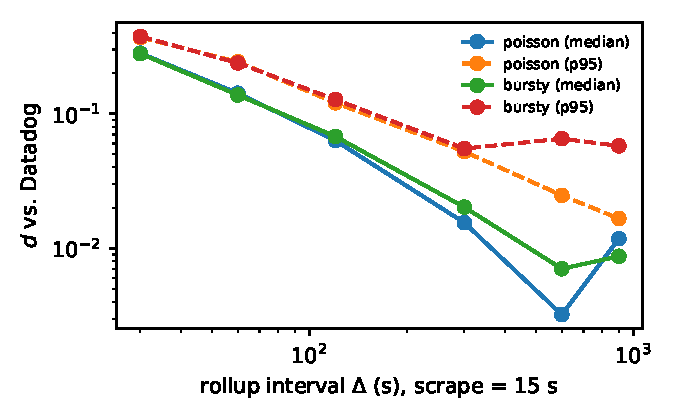
\includegraphics[width=0.6\linewidth]{figures/rate_error_vs_window}
\caption{Error of \texttt{rate()} against Datadog as the rollup interval grows, at a
$15$\,s scrape interval. \texttt{rate} is the only candidate whose error depends on the
data.}
\label{fig:rate-error}
\end{figure}

\subsubsection{The dual-write replay}
\label{sec:replay}

Everything to this point compares a PromQL candidate against our reading of Datadog's
rollup. That is a model, and a model is what \S\ref{sec:not-measured} warns the reader
about. This subsection closes the gap for the counter rules by running the dual-write
construction of this section literally: one stream of observations, written to both
systems, read back from both.

The stream is real. Counting the requests in a web-server access log into a scrape grid
gives a counter with the shape that \S\ref{sec:threats} says the synthetic workloads only
imitate: in the half hour used here the per-minute rate swings seventeenfold without
being asked to. We take the busiest half hour of the Kennedy Space Center HTTP logs of
July~1995~\citep{nasahttp}, count requests at a $15$\,s scrape interval into one counter
per HTTP status class, and write the cumulative series to Prometheus and its image under
$\phi_{\mathsf{zero}}$ --- the per-interval deltas --- to Datadog, at the same timestamps
(\texttt{scripts\slash replay\_dualwrite.py}).
The trace's publishers ask that it not be analysed beyond general traffic patterns, and
the parser enforces that rather than promising it: it keeps a timestamp and a status
class and discards the host and the request line, so what is replayed is a count of
requests per interval and nothing else. Timestamps are shifted to the present, because
Datadog's intake refuses points much older than an hour; the shape is real and the
absolute times are not.

\begin{table}[htbp]\centering\footnotesize
\begin{tabular}{@{}llrrr@{}}
\toprule
Scrape grid & PromQL candidate & Evaluated inside & On the edge & Max $d$ \\
\midrule
unaligned & \texttt{x - x offset $\Delta$} & 100.0\% & 100.0\% & 0 \\
 & \texttt{increase(x[$\Delta$] anchored)} & 100.0\% & 100.0\% & 0 \\
 & \texttt{rate(x[$\Delta$])} $\times\,\Delta$ & 20.2\% & 20.2\% & 1 \\
\addlinespace
aligned & \texttt{x - x offset $\Delta$} & 100.0\% & 27.4\% & 0 \\
 & \texttt{increase(x[$\Delta$] anchored)} & 100.0\% & 27.4\% & 0 \\
 & \texttt{rate(x[$\Delta$])} $\times\,\Delta$ & 20.2\% & 16.7\% & 1 \\
\addlinespace
\bottomrule
\end{tabular}

\caption{The dual-write replay: each candidate against \emph{Datadog}, bucket by bucket,
on a real request trace. ``Inside'' and ``on the edge'' are the two evaluation instants
of Remark~\ref{rem:closure}. $84$ comparisons per row.}
\label{tab:replay}
\end{table}

Table~\ref{tab:replay} is the result, and two things in it are worth separating.

The first is that both exact forms are exact --- against Datadog, not against a model of
it, on traffic nobody generated for the purpose. \texttt{rate} is not, at $20.2\%$ of
buckets on both grids, which is what \S\ref{sec:ingestion} has said throughout and what
the steady synthetic workload conceals by being steady. That figure used to read
$19$--$20\%$, a spread between the two grids that was not a property of either: the
replay script scored this one table by bit-identity where every other exactness column in
this paper uses a $10^{-12}$ relative bound, and one aligned bucket reading $236.0$
against $235.999\ldots$ counted as a disagreement.

The second is about the convention of Remark~\ref{rem:closure}, and it explains how that
convention came to be assumed wrongly for so long. On the unaligned grid --- a scrape
whose samples do not fall on rollup boundaries, which is what a jittered scrape produces
and therefore the ordinary case --- evaluating on the bucket's edge agrees with
evaluating inside it, on every bucket. Off a boundary the two half-open intervals contain
the same samples, so the closure is simply not observable. Snap the scrape grid onto the
rollup grid and the same comparison falls from $100\%$ to $27.4\%$. The error was
invisible in exactly the configuration real deployments have, and decisive in the one the
synthetic workloads of Table~\ref{tab:rollup-live} happen to use.

What this does not do is also worth stating. A request counter does not reset in half an
hour, so \texttt{COUNTER\_RESET} is not exercised here; the restart rows of
Table~\ref{tab:rollup-live} and the scripted reset of E1 (Remark~\ref{rem:rho}) are the
evidence for that case. It is one window of one
trace at one rollup interval. And it tests the counter rules, not translation coverage:
$\kappa$ is what it was.

\paragraph{What was assumed, and what is left.}
This section began with two facts about Datadog that its documentation does not settle,
and carried a third about its backend. None is still an assumption, and the two it began
with did not turn out the way they were guessed.

The reset policy $\rho$ is no longer among them either, and it is the one that was
settled twice: read from the agent's source and then put to a running agent, which
agreed with the reading (Remark~\ref{rem:rho}). It too went against the guess --- the
prediction recorded in advance was discarding the interval, which turns out not to be a
reset policy at all.

Bucket closure is no longer among them. Remark~\ref{rem:closure} settles it by
measurement: buckets are left-closed and named by their start, which is the opposite of
what an earlier draft of this section assumed and the opposite of PromQL's own
convention. Epoch alignment \emph{is} documented~\citep{ddrollup}, so the remaining
content of \texttt{ROLLUP\_ALIGNMENT} is sharper than ``align the grids'': a PromQL
window follows the evaluation step, and the step that reads a Datadog bucket is one
\emph{inside} its right edge rather than on it. Evaluating on the boundary --- the
obvious choice once the closure is known --- disagrees on every bucket where a scrape
lands on the boundary too, which is the ordinary case. The translator records
\texttt{ROLLUP\_ALIGNMENT} on every rollup it emits for that reason.

Nothing is left. The last of the three --- whether Datadog's backend stores what its
agent sends --- stood until a counter was made to reset on purpose, which is what the
replay above cannot do and what E1 does (Remark~\ref{rem:rho}). Both systems scrape one
endpoint across the reset; Datadog stores $103$ over the bucket holding it, and
\texttt{increase($x$[$60$s] anchored)} over Prometheus returns $103$ for the same bucket,
as it does on every complete bucket of all three counters. So the restart rows of
Table~\ref{tab:rollup-live} no longer stand alone: the anchored form tracks
$\phi_{\mathsf{zero}}$, and Datadog agrees with it where a counter actually restarts.

\iffull\apphead{What the vendor was asked}{app:experiments}

Datadog does not document the behaviour several of this paper's claims rest on, so it was
measured against a trial account and the raw responses cached under \texttt{data/raw/}.
The last of these asks the vendor's published integration repository rather than its API,
because what the dashboards omit that repository declares.
Each experiment below states its design, its prediction table where it has one, and what
came back; the body cites the answers.

\input{sections/moved/ing_closure_detail}
\input{sections/moved/ing_rho}
\input{sections/moved/ing_flush}
\input{sections/moved/ing_anchored_flag}
\input{sections/moved/tr_as_rate_placement}
\input{sections/moved/tr_gauge}
\input{sections/moved/tr_type_history}
\input{sections/moved/tr_type_measured}
\fi


\apphead{What the vendor was asked}{app:experiments}

Datadog does not document the behaviour several of this paper's claims rest on, so it was
measured against a trial account and the raw responses cached under \texttt{data/raw/}.
The last of these asks the vendor's published integration repository rather than its API,
because what the dashboards omit that repository declares.
Each experiment below states its design, its prediction table where it has one, and what
came back; the body cites the answers.

\begin{remark}[Which interval a bucket covers, measured]\label{rem:closure}
That the bucket is \emph{left}-closed and named by its \emph{start} is measured rather
than assumed, and it is not what we first assumed. Submitting one point at an exact
multiple of $\Delta$ and one strictly inside a bucket, and reading back which bucket each
is reported under, separates the four conventions: a point on a boundary is reported
under the bucket \emph{starting} there. Each of the other three conventions is ruled out
by at least one of the two readings (\texttt{scripts\slash trial\_checks.py e2}; the
responses are cached and regression-tested). It is one run at one rollup interval ---
the script fixes $\Delta$ at $60$\,s --- so what is pinned is the convention at that
width, not its independence of the width.

The convention PromQL uses for its own range selectors is the opposite one, $(u-w,u]$,
which is why it was the natural guess. Getting it wrong cost nothing numerically --- a
model and a candidate evaluated under the same convention agree with each other, so every
figure in Table~\ref{tab:rollup-live} is what it was --- but it was a claim about Datadog
that happened not to be true, and it changes where a translated query must be evaluated.
\end{remark}

\begin{remark}[Which $\rho$, and how we know]\label{rem:rho}
Datadog's documentation does not say what becomes of a counter decrease. Its agent is
open source, so the question can be answered by reading it~\citep{ddagent}, and then put
to a running one; both were done and they agree. The reading first.

The conversion carries a per-sample flag. With the flag set, a
sample below its predecessor contributes its own value, on the agent's stated assumption
that the counter restarted from zero --- this is $\delta_{\mathsf{zero}}$ term for term.
With the flag clear, the decrease contributes nothing and the point is still emitted,
which is $\delta_{\mathsf{clamp}}$. The OpenMetrics check sets the flag after every
successful scrape, so the ingestion path this paper models is $\phi_{\mathsf{zero}}$ from
its second scrape onward: the policy PromQL's own reset handling assumes.

Both branches above are thus implemented, and a third that an earlier draft of this
section offered --- discarding the interval outright --- is not, at least not as a reset
policy. Discarding is instead what happens at the \emph{start} of a series, where there is
no predecessor to difference against. A failed scrape is the interesting case: it clears
the flag, so the next interval is converted under $\mathsf{clamp}$ rather than
$\mathsf{zero}$, and is dropped altogether if the aggregator's stored predecessor has
expired in the meantime. Either way a transient failure perturbs $\phi(D)$ in a way
nothing applied to $D$ reproduces, and Proposition~\ref{prop:admissible} gives no warning,
because the discrepancy is between the two stored databases rather than between two
queries. No refusal can flag it and no translation can repair it.

Reading the agent establishes what it intends to send, not what the backend stores, and
the two are different claims. E1 closes the gap by putting a real agent in the loop. A
local endpoint exposes a counter that climbs by one per scrape to $1000$ and then, inside
one rollup bucket, drops to $100$; a Datadog Agent runs an OpenMetrics check against it
and a Prometheus scrapes the same endpoint. Over the bucket holding the reset Datadog
stores $\mathbf{103}$ across four points --- the increment before the reset, the new
value reported as the reset interval's own count, and the two increments after it. That
is $\delta_{\mathsf{zero}}$ and nothing else: $\mathsf{clamp}$ predicts $3$ over four
points, discarding the interval predicts $3$ over three, and a backend keeping the signed
difference predicts $-897$. The four predictions were recorded before the run and are
regression-tested in \texttt{tests\slash test\_reset.py}. A second counter resetting to
exactly $0$ rather than $100$ reads $3$, which is what $\mathsf{zero}$ requires and rules
out a special case at zero; a third that never resets reads four increments of one in
every bucket, which is what shows the run is reading the bucket it means to.
\end{remark}

\begin{remark}[$\phi_\rho$ and the flush interval]\label{rem:flush}
$\phi_\rho$ differences consecutive \emph{samples}, and the agent aggregates samples
into the interval it flushes. An earlier version of this remark inferred from the source
that the two part company as soon as a flush holds more than one sample: a decrease
appeared to \emph{overwrite} what the interval had accumulated rather than adding to it,
so a flush holding an increase and then a reset should report the post-reset value alone,
where $\phi_{\mathsf{zero}}$ keeps both. The agent's default scrape and flush intervals
are both $15$\,s, which would make the question moot in the default configuration and
was the reason it went untested.

Put to a running agent, it does not happen --- though not quite for the reason the run
was designed to test, and the difference is worth keeping. Driving the OpenMetrics
check at a $5$\,s collection interval against the unchanged $15$\,s flush, the bucket
holding the reset reports $111$: eleven increments of one and the reset's own value,
which is $\phi_{\mathsf{zero}}$ term for term. Losing the increment that shares a flush
with the reset would give $110$ (\texttt{scripts\slash reset\_policy.py -{}-step 5}).

What the stored data then shows is that no flush combined anything. Every complete
$60$\,s bucket holds twelve points, one per collection, where three samples to a flush
would have left four. So the agent forwarded each sample rather than aggregating within
the flush, and the overwrite this remark used to posit had no opportunity to occur. The
hypothesis is therefore unexercised rather than refuted, and what the run does
establish is the end-to-end fact the exactness claims actually use: at this ratio
Datadog stores $\phi_{\mathsf{zero}}$ term for term, so those claims do not depend on
the scrape and flush intervals agreeing. The ratio itself was configured and not
observed --- the record computes it from the two interval settings --- and no run here
drives it to a point where a flush must combine samples.
\end{remark}

\begin{remark}[\texttt{anchored} is still experimental]\label{rem:anchored-flag}
The \texttt{anchored} modifier of~\citet{prom0052} arrived in Prometheus~3.7.0 behind
\texttt{-{}-enable-feature=promql-extended-range-selectors}, and an earlier draft of this
section asserted that the flag had since become a no-op. It has not. A $3.15.0$ server
started without it rejects the expression outright:
\begin{center}\footnotesize
\texttt{anchored modifier is experimental and not enabled}
\end{center}
The precondition \texttt{ANCHORED\_VERSION} records is therefore stronger than a version
number. It is a server deliberately started with an experimental feature enabled, which
is a different and larger ask of whoever operates the target: a version can be waited
for, a flag has to be chosen. That is the real cost of
Proposition~\ref{prop:anchored}'s exactness, and it is the reason the emitter leaves the
reset-aware form off by default and emits the cumulative difference, which uses nothing
outside standard PromQL.

The error above is how we found out. Every measurement in this paper had been taken with
the flag set, because the script that takes them passes it and a comment there described
it as harmless; the claim was never exercised until a later experiment started a server
without it. A precondition that every instrument satisfies by habit is one nobody tests.
\end{remark}

\begin{remark}[Where \texttt{.as\_rate()}'s divisor sits]\label{rem:as-rate-placement}
The rollup is inside the space aggregation and the modifier's division is not, which is
a second ordering question and was answered the same way round as the first: wrongly, at
first, and then by measurement.

\texttt{.as\_rate()} divides by the rollup interval. Dividing by a positive constant
commutes with $\mathsf{sum}$, $\mathsf{avg}$, $\mathsf{min}$ and $\mathsf{max}$, so for
those the divisor can sit on either side of the space aggregation and nothing
distinguishes the readings. It does not commute with $\mathsf{count}$, which counts
series and is blind to their values: $\mathrm{count}(x/\Delta) = \mathrm{count}(x)$
while $\mathrm{count}(x)/\Delta$ is not. So one operator decides the question for all
of them, and asking it of a real account answers it ---
\texttt{count:m\{*\} by \{g\}.rollup(avg, 30)} returns $1$ per group and the same
query with \texttt{.as\_rate()} returns $1/30$
(\texttt{scripts\slash as\_rate\_order.py}). Datadog divides the aggregated result, so
the emitter places the divisor outside the aggregation for $\mathsf{count}$ and, for
readability, leaves it inside where it commutes.

The same run settles the modifier's other ordering, against an explicit
\texttt{.rollup}. Submitting every $10$\,s and rolling up over $30$\,s separates
dividing each delta by its own submission interval from rolling up and dividing once by
the bucket: the first reads $1$, the second $10/30$. Datadog reads $10/30$. Both
readings coincide whenever the submission grid equals the rollup width, which is every
harness in this project and the reason the question went unasked for so long.
\end{remark}

\begin{remark}[The assumption that underwrites all of the output]%
\label{rem:gauge}
Writing Theorem~\ref{thm:kernel} down is what exposed this. An
$\mathit{op}\in\{\mathsf{avg},\mathsf{min},\mathsf{max},\mathsf{count}\}$ rollup reduces
the points Datadog \emph{stores}. For a GAUGE those are the samples Prometheus also
holds, and \texttt{avg\_over\_time(x[$\Delta$s])} is exact. For a COUNT they are
per-interval deltas, and averaging deltas is not averaging running totals --- no
\texttt{*\_over\_time} of the cumulative series computes it, and the emitted expression is
not approximately right but unrelated. The dashboard never says which, so the emission is
correct for a gauge and the emitter records \texttt{METRIC\_TYPE\_UNKNOWN} to say so. It
reports rather than refuses
because a rule \emph{can} be chosen here; for a $\mathsf{sum}$ rollup none can, and the
same code is a refusal there instead.

The condition is not a precaution. Asked of a real account, a bare query on a
\texttt{COUNT} metric returns the \emph{mean} of four stored deltas,
so Datadog applies its enforced \texttt{avg} default rather than the \texttt{.as\_count()}
its user interface appends --- averaging deltas where \texttt{avg\_over\_time} averages
running totals (\texttt{scripts\slash trial\_checks.py e3}). The deltas are $1$, $14$,
$2$ and $3$, chosen so that each candidate predicts a different reading: $\mathsf{avg}$
gives $5$, $\mathsf{sum}$ gives $20$, a $\mathsf{count}$ rollup gives $4$ and
$\mathsf{sum}$ over the reported interval gives $1$. The account returns $5$. The first
version of this probe used $1$, $2$, $3$ and $10$, whose mean is $4$ and whose count is
also $4$, and named $\mathsf{avg}$ against a rival set that did not include
$\mathsf{count}$ --- so the reading it took could not have told the two apart.

The condition was also silent until now, and it is not rare. At an earlier stage of this
work it appeared to hold of $6{,}381$ translated occurrences --- $76.2\%$ of the
translated set as it then stood, which was smaller than today's --- because Datadog's
default time aggregator is $\mathsf{avg}$ and most queries state no method at all. The remaining quarter looked exempt: a $\mathsf{sum}$ rollup needs a
counter, the ways to ask for one are \texttt{.as\_count()}, \texttt{.as\_rate()} and
\texttt{.rollup(sum, $\Delta$)}, and all three are documented for \texttt{COUNT}
metrics --- so a query using one, we reasoned, establishes the type it does not state.

It does not, and the error was of a kind this paper has made before: a rule read in a
manual and never asked of the system. Submitting a \texttt{GAUGE} and querying it with
each modifier returns the plain rollup, unchanged and undivided --- Datadog accepts both
on a gauge and silently ignores them rather than rejecting the query
(\texttt{scripts\slash as\_rate\_order.py}). The modifier therefore records what the
dashboard's author took the metric to be. It is evidence about a person, not about a
type, and no reading of the query distinguishes the two.

The third way is weaker still, and for a different reason. \texttt{.rollup(sum, $\Delta$)}
over a \texttt{GAUGE} is not ignored: the same experiment reads it as the sum of the
stored samples, which is a perfectly meaningful query that a dashboard author might well
intend. So where \texttt{.as\_count()} on a gauge is a mistake nobody benefits from,
summing a gauge over a window is an ordinary thing to want --- and the translation this
front end chooses for it, the cumulative difference, computes something else entirely.
Of the three pieces of evidence the query can carry, the one that is hardest to dismiss
as author error is the one whose misreading is least benign. With that premise withdrawn the
caveat holds of all $8{,}475$ translated occurrences, $100\%$ of them
(Table~\ref{tab:translation-caveats}).

Recording it does not move $\kappa$ --- the translations are unchanged --- which is the
point: it changes what they are claimed to be. Its refusing counterpart still never fires,
but for a weaker reason than the one we gave: not because the method establishes the type,
but because it is the only syntax that asks for the rule, so the emitter always has a rule
to choose and never has to stop. So the same unstated fact is a diagnostic that cannot
occur and a precondition that always does.
\end{remark}

\begin{remark}[What hypothesis~(3) costs when it fails]\label{rem:type-cost}
Hypothesis (3) is the one that changed shape while this paper was being written, and
twice. It began as ``the metric is a gauge'', which was the only case the emitter then
handled; a counter under an averaging rollup was being emitted as
\texttt{avg\_over\_time} of the running totals, which is not a function of the deltas
Datadog reduces at all, and the corpus-scale differential test of \S\ref{sec:differential}
is what caught it. It then stopped being dischargeable from the query text, when the
modifiers it rests on turned out not to establish the type (Remark~\ref{rem:gauge}).
What it costs when it fails is measured rather than asserted: writing one stream of
counter observations to both systems and asking the commonest shape in the corpus ---
a query with no method at all --- Datadog reads the mean of the deltas, $10$ throughout,
while \texttt{avg\_over\_time} reads the mean of the running totals, climbing from $20$
to $1{,}760$ over half an hour. The relative difference runs from $0.50$ to $0.994$ and
is unbounded in the counter's age, because one quantity grows with it and the other does
not. The same run with the metric submitted as a \texttt{GAUGE}, where the hypothesis
holds, agrees exactly on every bucket (\texttt{scripts\slash type\_assumption.py}).
\end{remark}

\begin{remark}[How often the inference is wrong]\label{rem:type-measured}
A precondition that holds of all the output and cannot be checked is the weakest thing
this paper carries, and it turns out to be checkable. The dashboards do not record a
metric's type --- but the repository they come from does. Beside each integration's
\texttt{assets\slash dashboards\slash}, \texttt{integrations-core} ships a
\texttt{metadata.csv} with a \texttt{metric\_type} column, and
\texttt{scripts\slash fetch\_corpus.py} had taken only the dashboards.
\texttt{scripts\slash fetch\_metric\_types.py} fetches the rest, reading the commit
from the corpus's own record so the declarations cannot come from a different tree than
the queries. At that commit those files declare $37{,}070$ metric names: $23{,}597$
\texttt{gauge}, $13{,}140$ \texttt{count}, $330$ \texttt{rate} and three that two
integrations declare incompatibly.

Joining the two settles the hypothesis for most of the corpus
(\texttt{scripts\slash type\_declared.py}). Of the $8{,}444$ translated occurrences,
$7{,}557$ --- $89.5\%$ --- name a metric the repository declares as a gauge or a count,
and the front end's inference disagrees with the declaration on $491$ of them: $6.5\%$
of the decidable set, $5.6\%$ of the corpus. The two directions of error are both
present and are different failures. In $242$ occurrences the metric is a
\texttt{count} and the query carries no evidence of it, so the emitter translates it as
a gauge and the \texttt{*\_over\_time} it produces reduces running totals where
Datadog reduces deltas --- the case this remark describes as unrelated rather than
approximate. In $249$ the metric is a \texttt{gauge} and the query carries
\texttt{.as\_count()}, \texttt{.as\_rate()} or \texttt{.rollup(sum, $\Delta$)}
anyway, so the evidence is not merely weak but actively wrong, and the emitter chooses
a counter rule for a series that has no deltas to difference.

What this is evidence of, and what it is not. \texttt{metadata.csv} states what an
integration submits, so a disagreement says the inference is wrong, not that it must
be: a dashboard can query a metric the integration does not ship, and an operator can
submit the same name as something else. That is the same standard \S\ref{sec:emission}
applies to the modifier evidence this replaces, and it is a sharper instrument than the
one it replaces rather than a proof. The remaining $887$ occurrences divide three ways: $736$ name metrics the
repository does not declare, $134$ name \texttt{rate} metrics --- a third
submission type Definition~\ref{def:phi} maps by the identity rather than modelling ---
and $17$ name one of the three metrics two integrations declare incompatibly, so the
repository states a contradiction rather than a type.
\end{remark}


\apphead{Corpus and evaluation apparatus}{app:eval}

What the corpus is made of beyond the counts \S\ref{sec:evaluation} quotes, how the
feature-coverage order is computed, and the two subsections that report what the
evaluation does \emph{not} establish. The body carries the answers; this carries the
characterisation a reader would need to disagree with them.

\begin{remark}[Two definitions in one comparison]\label{rem:template-shares}
The two template-variable shares beside the parse rates are now the same quantity, and
were not. The Datadog figure used to read $87\%$, which is the share of queries with a
variable \emph{inside a scope} and not the share with a variable at all, while the PromQL
figure beside it was the latter --- two definitions in one comparison, and the narrower
one on the side the sentence was about. A comparison between two languages is the place a
definitional slip is hardest to see, because the number it produces is of the right order
and points the way the argument already pointed.
\end{remark}

\begin{remark}[Three counts that moved on a seventh reading of the extractor]\label{rem:extraction-fixes}
Three of those counts moved in the seventh reading of the extractor, and in the direction
that costs an excuse rather than buying one: a request may carry its query as a singular
object rather than in a list, which distribution widgets do and which hid four Datadog
queries; a Grafana library panel keeps its model in the dashboard's \texttt{\_\_elements}
map rather than in \texttt{panels}, which hid four more; and \emph{two} of what had been
eleven LogQL panels were PromQL alerting rules whose only offence was a backtick raw
string in a matcher, which PromQL permits and a LogQL line-filter pattern matched.
\end{remark}

\paragraph{What is held aside.}
A Datadog widget is a list of named queries plus a formula over them, and this paper is
about the metrics query language rather than the formula layer. Scoping it out is cheap
and the corpus says so: of $6{,}022$ formulas ($444$ distinct strings), $75.6\%$ are a
bare reference to a single named query, $13.8\%$ apply one function, $13.2\%$ contain
arithmetic and $8.2\%$ a numeric constant. The semantics sit in the queries, not above
them.

The population is the metric formula layer and not the whole of it, which is the
correction the sentence above needed. A formula sits over a request's queries, so it
belongs to the metrics language only when they do, and the extractor applied that filter
to the queries and not to the formulas. The $11{,}628$ formulas an earlier version of
this paragraph reported were $6{,}022$ metric ones and $5{,}606$ over log, event,
security-signal and other requests --- and the second group is $90.1\%$ bare references,
so it diluted every share here towards the answer the paragraph wanted. Arithmetic in the
formula layer is nearly twice what was claimed. The conclusion survives: three quarters of
the metric formula layer is a name, and nothing in it computes what a query cannot.

\paragraph{What the corpus is not.}
It is a census of \emph{published} dashboards, not of production estates. Vendor
integration dashboards are written to demonstrate an integration, and community
dashboards are written to be shared, so both are plausibly tidier and more
template-driven than a dashboard grown inside one company. The direction of that bias is
not obvious --- a tidier corpus is easier to parse but no easier to translate --- and
Section~\ref{sec:threats} returns to it.


\subsection{What the two languages are used for}

A grammar says what is sayable. The corpus says what is said, and the distributions are
lopsided enough to change what a translator should be built out of.
Figure~\ref{fig:feature-frequency} gives the structural features and
Table~\ref{tab:operator-frequency} the operators.

\begin{figure}[htbp]\centering
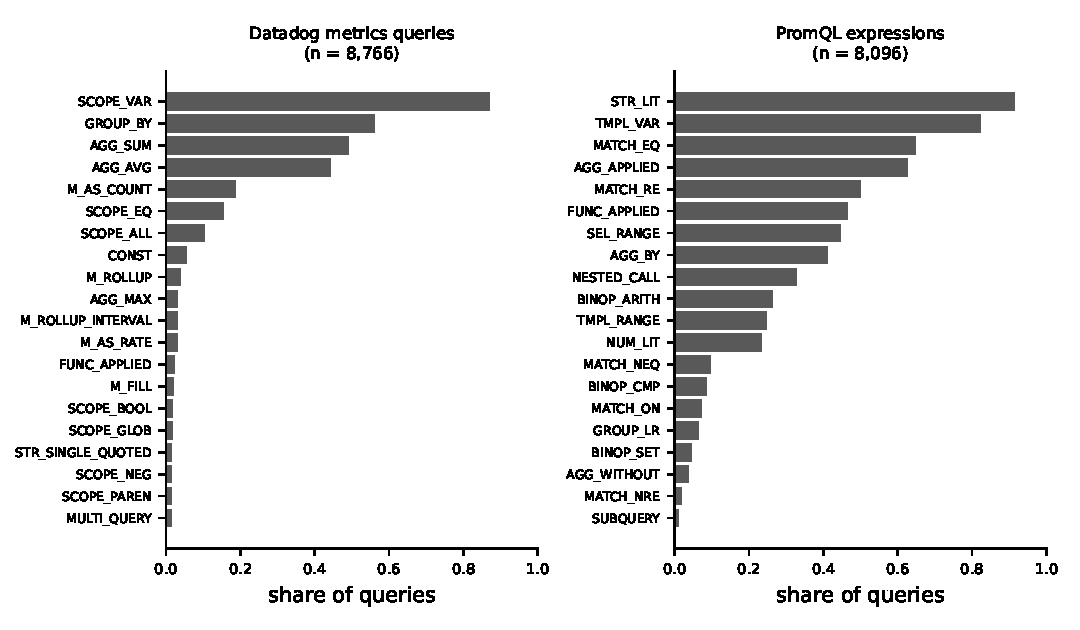
\includegraphics[width=\linewidth]{figures/feature_frequency}
\caption{The twenty most frequent structural features per language, as a share of
queries. Feature codes are those of \texttt{corpus.FEATURE\_DOC}; a query contributes to
every feature it uses.}
\label{fig:feature-frequency}
\end{figure}

\begin{table}[htbp]\centering\footnotesize
\begin{tabular}{@{}lllr@{}}
\toprule
Language & Kind & Name & Occurrences \\
\midrule
datadog & aggregator & \texttt{sum} & 4,480 \\
datadog & aggregator & \texttt{avg} & 4,057 \\
datadog & aggregator & \texttt{max} & 275 \\
datadog & aggregator & \texttt{count} & 58 \\
datadog & aggregator & \texttt{min} & 51 \\
datadog & aggregator & \texttt{p95} & 19 \\
datadog & function & \texttt{.as\_count} & 1,766 \\
datadog & function & \texttt{.rollup} & 331 \\
datadog & function & \texttt{.as\_rate} & 266 \\
datadog & function & \texttt{.fill} & 185 \\
datadog & function & \texttt{top} & 163 \\
datadog & function & \texttt{.weighted} & 70 \\
datadog & function & \texttt{per\_minute} & 27 \\
datadog & function & \texttt{per\_second} & 22 \\
datadog & function & \texttt{derivative} & 15 \\
datadog & function & \texttt{count} & 8 \\
promql & aggregator & \texttt{sum} & 4,718 \\
promql & aggregator & \texttt{max} & 718 \\
promql & aggregator & \texttt{avg} & 621 \\
promql & aggregator & \texttt{count} & 307 \\
promql & aggregator & \texttt{topk} & 230 \\
promql & aggregator & \texttt{min} & 84 \\
promql & function & \texttt{rate} & 2,541 \\
promql & function & \texttt{irate} & 1,078 \\
promql & function & \texttt{histogram\_quantile} & 507 \\
promql & function & \texttt{increase} & 328 \\
promql & function & \texttt{label\_replace} & 152 \\
promql & function & \texttt{vector} & 113 \\
promql & function & \texttt{sort\_desc} & 91 \\
promql & function & \texttt{label\_join} & 55 \\
promql & function & \texttt{time} & 50 \\
promql & function & \texttt{round} & 46 \\
\bottomrule
\end{tabular}

\caption{The six most frequent space aggregators and ten most frequent functions per
language, by occurrence. Datadog's \texttt{p}$NN$ percentile aggregators are five
distinct operators totalling $34$ occurrences, of which only \texttt{p95} reaches this
table.}
\label{tab:operator-frequency}
\end{table}

\noindent
Four things in these distributions are load-bearing for the rest of the paper.

\emph{Datadog's head is very short.} \texttt{sum:} and \texttt{avg:} are $95\%$ of all
every space-aggregator occurrence in Table~\ref{tab:operator-frequency}, and \texttt{by \{...\}} appears in $56\%$ of
queries. A translator that handles two aggregators and grouping already speaks most of
what the corpus says.

\emph{The counter rule that matters is the undivided one.} \texttt{.as\_count()} outnumbers
\texttt{.as\_rate()} by $6.6$ to one ($1{,}766$ against $266$). Both reduce to the same
cumulative difference by Proposition~\ref{prop:offset}, which is why that proposition,
rather than anything about \texttt{rate}, is the one that carries a migration.

\emph{PromQL's head is a rate.} \texttt{rate} and \texttt{irate} together are $69\%$ of
all $5{,}227$ function occurrences. Meanwhile subqueries appear in $1.1\%$ of PromQL
queries, \texttt{offset} in $0.3\%$, and the \texttt{@} modifier in none at all --- a
construct the language has and $8{,}096$ shipped expressions never reach for. The gap
between what a query language contains and what its users employ is itself part of the
switching-cost story: the hard parts of a language can be rare.

\emph{Nothing is used alone.} A real Datadog query combines a space aggregator, a scope
of several terms, a grouping and at least one method. That is why marginal frequency is
the wrong order to build a translator in, and why the next subsection reports a different
order.


\subsection{Coverage is a staircase, not a curve}
\label{sec:staircase}

A query is translatable only when \emph{every} feature it uses is supported, so for a
translator supporting exactly the feature set $S$, the share of queries all of whose
features lie in $S$ is an upper bound on $\kappa$. Choosing $S$ greedily --- at each step
the feature that completes the most queries outright --- gives an attainable set at each
size, hence a lower bound on the best ceiling a fragment of that size could reach.
Table~\ref{tab:implementation-order} is that order for Datadog and
Figure~\ref{fig:cumulative-coverage} both curves.

\begin{table}[htbp]\centering\scriptsize
\begin{tabular}{@{}rllrrr@{}}
\toprule
Step & Feature & Construct & Pending uses & Queries completed & Cumulative \\
\midrule
1 & \texttt{GROUP\_BY} & group by \{...\} & 4,922 & 20 & 1\% \\
2 & \texttt{MULTI\_QUERY} & comma-separated list of queries & 117 & 9 & 1\% \\
3 & \texttt{ARITH} & arithmetic between operands & 115 & 5 & 2\% \\
4 & \texttt{CONST} & numeric literal & 470 & 9 & 2\% \\
5 & \texttt{FUNC\_APPLIED} & function applied to the query & 205 & 1 & 2\% \\
6 & \texttt{AGG\_AVG} & space aggregator avg: & 3,885 & 1 & 2\% \\
7 & \texttt{SCOPE\_VAR} & dashboard template variable in the scope & 7,624 & 2,468 & 30\% \\
8 & \texttt{AGG\_SUM} & space aggregator sum: & 4,314 & 1,708 & 49\% \\
9 & \texttt{M\_AS\_COUNT} & .as\_count() & 1,644 & 1,079 & 62\% \\
10 & \texttt{SCOPE\_EQ} & scope term key:value & 1,347 & 974 & 73\% \\
11 & \texttt{SCOPE\_ALL} & scope \{*\} & 898 & 810 & 82\% \\
12 & \texttt{AGG\_MAX} & space aggregator max: & 275 & 245 & 85\% \\
13 & \texttt{M\_AS\_RATE} & .as\_rate() & 266 & 224 & 87\% \\
14 & \texttt{STR\_SINGLE\_QUOTED} & single-quoted string literal & 139 & 136 & 89\% \\
15 & \texttt{M\_FILL} & .fill(...) & 185 & 94 & 90\% \\
16 & \texttt{SCOPE\_GLOB} & wildcard in a scope value & 143 & 89 & 91\% \\
17 & \texttt{SCOPE\_NEG} & negated scope term !key:value & 134 & 91 & 92\% \\
18 & \texttt{M\_WEIGHTED} & .weighted() & 70 & 64 & 93\% \\
19 & \texttt{AGG\_COUNT} & space aggregator count: & 58 & 53 & 93\% \\
20 & \texttt{SCOPE\_BOOL} & boolean scope (AND / OR / NOT) & 160 & 37 & 94\% \\
\bottomrule
\end{tabular}

\caption{Greedy implementation order for Datadog. ``Pending uses'' is how many queries
still need the feature when it is chosen; ``queries completed'' how many it finishes on
its own. The cumulative column bounds $\kappa$ for a translator limited to those
features.}
\label{tab:implementation-order}
\end{table}

\begin{figure}[htbp]\centering
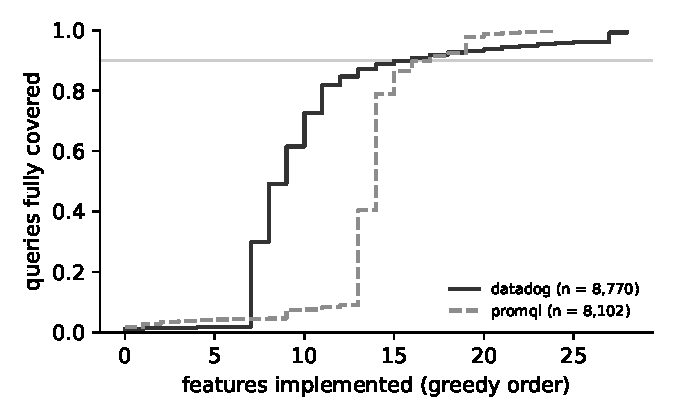
\includegraphics[width=0.62\linewidth]{figures/cumulative_coverage}
\caption{Queries fully covered against features implemented, in greedy order. The line
at $0.9$ marks the level reached after sixteen of Datadog's twenty-eight features and
seventeen of PromQL's twenty-four.}
\label{fig:cumulative-coverage}
\end{figure}

The shape is the finding. The first six Datadog features complete $45$ queries between
them --- $0.5\%$ of the corpus, on top of the $1.1\%$ that use no feature at all --- and
then template-variable scopes and \texttt{sum:} take two steps to $49.2\%$. Half the corpus
needs nine features; $90\%$ needs sixteen of the twenty-eight. PromQL behaves the same way
and slightly worse: its first six features complete $221$ of $8{,}102$ queries
($2.7\%$), half the corpus needs fourteen features and $90\%$ needs seventeen of
twenty-four.

For anyone building one of these translators this is the practical result of the paper. A
partial translator is worth almost nothing: there is no prefix of the feature list that
buys proportional coverage, because coverage is conjunctive over features while
popularity is marginal. The ``$80\%$ of queries with $20\%$ of the work'' intuition is
simply false here, and that asymmetry is a switching cost in its own right --- an
incremental migration cannot show incremental progress.


\subsection{What the unparsed queries are}

Six distinct queries ($8$ occurrences) are outside the grammar of
Section~\ref{sec:grammars}, and all six are the same construct: a conditional aggregator,
\texttt{count(v: v>=0):data\_streams.latency\{...\}}, which appears in Datadog's own
shipped dashboards and in none of its documentation. Writing a production for it would
mean guessing its semantics, so it is reported instead. It is the whole of the Datadog
residual in Table~\ref{tab:parse-coverage}.

\subsection{What is not measured}
\label{sec:not-measured}

Two of the facts this paper's rollup translations rest on are facts about Datadog's
implementation rather than about either language, and Datadog's documentation settles
neither. They are stated as assumptions in Section~\ref{sec:ingestion} and carried as
diagnostics in Table~\ref{tab:translation-caveats}. Both have since been settled, one of
them first from a source other than an experiment and then by one, and the difference
between the two kinds of evidence is worth keeping visible.

\emph{The reset policy $\rho$, settled by reading and then by measurement.} Datadog's
agent is open source, so what it does with a counter decrease is readable even though it
is undocumented: Remark~\ref{rem:rho} establishes $\rho=\mathsf{zero}$ for the
OpenMetrics ingestion path, which is what Proposition~\ref{prop:anchored} assumes. This
was not the expected answer. The prediction recorded in advance was
$\rho=\mathsf{drop}$, on which \emph{neither} candidate would have been exact across a
reset; the policy that the agent does implement alongside $\mathsf{zero}$ turns out to be
$\mathsf{clamp}$, and $\mathsf{drop}$ is not a reset policy at all.

Reading the agent does not establish that the backend stores what the agent sends, and
that step stood open longer than any other in this paper --- not for want of a design,
but because the experiment needs a counter that resets, and the replay of
Section~\ref{sec:replay} cannot supply one: a real request counter does not restart
inside half an hour. E1 supplies one on purpose. A scripted counter climbs to $1000$ and
drops to $100$ inside a single bucket while a real agent and a real Prometheus scrape the
same endpoint. Datadog stores $103$ over that bucket, which is $\delta_{\mathsf{zero}}$
and is distinct from what each of the three rivals predicts; and
\texttt{increase(x[$\Delta$] anchored)} over Prometheus returns $103$ for the same
bucket, on every complete bucket of all three counters. The restart rows of
Table~\ref{tab:rollup-live} therefore no longer stand on the model alone.

\emph{Bucket closure, settled by measurement.} $\Sigma_\Delta$ presumes a bucket
convention, and the one it presumed was wrong. Submitting a point on an exact bucket
boundary and another strictly inside one, then reading back which bucket each is reported
under, shows the buckets are left-closed and named by their \emph{start}
(Remark~\ref{rem:closure}); the two probes together leave one convention standing, and
each rival is ruled out by at least one of the two readings. It is one run at one rollup
interval, as \S\ref{sec:ingestion} says and this subsection used to deny by claiming two
runs at two intervals --- so what is pinned is the convention at $60$\,s rather than its
independence of the width. Epoch alignment itself \emph{is}
documented~\citep{ddrollup}; which edge the timestamp names was not.

No figure in this paper moved. A model and a candidate evaluated under the same
convention agree with each other, so what was wrong was a claim about Datadog rather than
any arithmetic --- Table~\ref{tab:rollup-live}, recomputed against a freshly re-verified
Prometheus on the corrected grid, is identical to the version computed under the wrong
one. What did change is where a translated query must be evaluated, and that is not a
detail: since a PromQL window is right-closed, no instant reads a left-closed bucket
exactly when a scrape lands on a boundary, and the translation must be evaluated strictly
inside the bucket. Evaluating on its right edge --- the obvious repair once the closure is
known --- is wrong on almost every bucket of an aligned scrape.

\emph{The corpus-scale differential test, no longer outstanding.} One further item
belonged in this subsection until recently, and it was the largest of them: the
construction of Section~\ref{sec:replay} applied to the whole corpus rather than to one
replayed trace. Until it ran, $\kappa$ measured what the translator was willing to
translate rather than what it translated correctly. It has since been run, and
\S\ref{sec:differential} reports it --- named rather than pointed at, because this
block is inline in one build and the last subsection of an appendix in the other,
where ``the next subsection'' was the references.



\texttt{UNSUPPORTED\_FUNCTION} is the largest and the least interesting: it is mostly a
bundle of Datadog functions the translator does not implement. \texttt{top(...)} leads
it at $139$ occurrences, and \texttt{per\_second(...)} follows at $22$.
Mostly, and not wholly: $11$ of its $208$ are not functions at all. Nine are a negated match-all,
\texttt{\{*,!*\}}, which is a scope and which the catalogue's own shortest example for
this row happens to be; one is a \texttt{.rollup(max)} over a known counter, which the
proof of Theorem~\ref{thm:kernel} classifies as a case where no rule exists rather than
as unwritten code; and one is a rollup whose \emph{width} is not numeric,
\texttt{.rollup(count, daily)}, refused where the interval is parsed rather than where a
function is looked up. All three stay in the unimplemented column, though the first of them for a duller
reason than \S\ref{sec:gaps} first gave: an earlier draft argued that PromQL can
denote an empty selection with a contradictory matcher pair and that \texttt{\{*,!*\}}
asks for one. The first is true and the second is false
(Remark~\ref{rem:empty-tag}) --- the term is discarded, and the exact translation is
to drop it. The individual deltas a
\texttt{max} rollup needs are reachable through a subquery over a sample grid the
query does not state --- the same omission the rollup interval makes everywhere else
--- and a
named calendar width is a unit the front end does not yet convert. Everything in it is now unimplemented
work and nothing else, which it was not when this section was first written: the
percentile aggregators sat in it as a genuine gap and \texttt{.weighted()} as a
supposed one, so the row was a mixture and the split at the end of this subsection had
to be computed by reading detail strings rather than codes. Both have moved ---
\texttt{.weighted()} out of the catalogue entirely (Remark~\ref{rem:weighted}) and the
percentiles into a code that names their obstruction.

The converse does not hold, and the comparison this subsection ends with depends on
noticing it: this row is not the whole of the unimplemented column. That column is now
five codes and $287$ occurrences --- this row's $208$, the four surviving disjunctions
below, the $36$ \texttt{FILL\_INTERPOLATION} occurrences Remark~\ref{rem:fill} moved
into it, and the $34$ \texttt{PHI\_QUANTILE} and $5$ \texttt{SCOPE\_EMPTY\_VALUE}
occurrences \S\ref{sec:gaps} moved into it last. This sentence read ``this row's $208$,
those four, and the $36$'' for as long as the column had held three codes, which sums to
$248$ and not to $287$: the last two retractions added their occurrences to the column
and not to the sentence describing it. One code has stopped being a mixture; the column
spans five, and it is the column rather than the code that the comparison is about.


\begin{remark}[\texttt{.weighted()} was the largest claimed gap and is not one]%
\label{rem:weighted}
Until recently this row was led by \texttt{.weighted()} at $70$ occurrences, described
here as ``a time-weighted space average that PromQL has no operator for''. That sentence
was the entire warrant, and it was wrong in both halves.

It is not an average: all $52$ distinct corpus forms attach the modifier to
\texttt{sum:}. An earlier version of this remark said $54$ of $56$ and conceded two
\texttt{avg:} uses; there are none. The count came from matching the substring
\texttt{weighted}, which also catches four queries whose \emph{metric name} contains it
and which carry no modifier at all --- two of them \texttt{avg:}, which is exactly the
concession. And it is not a gap, because it does not compute anything. A series
reporting at $0$, $50$ and $55$ seconds into each $60$\,s bucket has a plain mean of
$66.7$ and a mean weighted by the interval each point covers of $16.7$, so a rig built
on it can tell the two apart. Datadog returns $66.7$ with the modifier and without it,
on \texttt{GAUGE}, \texttt{COUNT} and \texttt{RATE} alike
(\texttt{scripts\slash weighted\_semantics.py}). The probe is narrower than that list
makes it sound, and the gap is worth naming: the grouped forms and the \texttt{sum} and
\texttt{avg} rollups were run on the gauge only, the counter types were probed
ungrouped under \texttt{avg}, and the modifier was never paired with a \texttt{count}
rollup at all. What closes that is not the probe but the corpus: three
\texttt{.weighted()} shapes went through the differential of \S\ref{sec:differential}
and agreed with Datadog bucket for bucket. On everything this corpus does with it,
\texttt{.weighted()} is the identity.

So the translation of a query carrying it is the translation of the query without it,
the front end drops the modifier as it already dropped \texttt{.fill(null)}, and $70$
occurrences move from the inexpressible column to $\kappa$. That is the third claimed
language gap in this paper to turn out not to be one, and the first to turn out not to
be work either: the other two were implemented, and this one needed deleting. The residue is a caution rather than a result: a modifier that does nothing
everywhere we can look may still do something somewhere we cannot, and what is measured
is every metric type and query shape the rig can build, not every configuration Datadog
has.
\end{remark}


\texttt{top(...)} decides where that split falls, so it is worth settling rather than
asserting. An earlier draft of this paragraph called it ``close to PromQL's
\texttt{topk}'', and that is false: Datadog ranks series by an aggregation over
\emph{all} values in the queried range and returns those series' whole trajectories,
while \texttt{topk} ranks independently at each evaluation instant, so a series can be in
one and not the other. They are different operators, and $139$ occurrences moving into
the inexpressible column would invert the comparison this section ends with.

They do not move, and the reason is instructive. PromQL \emph{can} denote the ranking,
using the \texttt{@} modifier to pin it to a single evaluation so that it does not drift
across the graph:
\begin{center}\footnotesize
\texttt{q and on($\overline{k}$) topk($n$, max\_over\_time(q[$R$] @ $T$))}
\end{center}
Read off a real Prometheus~3.15.0, this reproduces the selection that Datadog's
documented rule predicts --- aggregate each series over the whole range, take the top
$n$ --- and holds it constant across the range, while the naive \texttt{topk($n$, q)}
changes membership within the same workload at $n=2$
(\texttt{scripts\slash verify\_topk.py}; cached and regression-tested).
All $20$ cases agree: five ranking
functions, at $n=2$ and $n=3$, in both directions. The directions were the omission worth
finding. This corpus ranks ascending in $5$ of its $139$
occurrences, \texttt{topk} is the descending half of \texttt{top()}, and until
\texttt{bottomk} was asked for as well the measurement covered $134$ occurrences while
the sentence reporting it claimed $139$. The functions run the other way: the probe
covers five and the corpus uses four --- \texttt{mean} in $111$ of the calls,
\texttt{last} in $34$, \texttt{max} in $15$ and \texttt{sum} in $3$ --- so \texttt{min}
is probed because the candidate has to hold for it, not because a dashboard asks.

The Prometheus reading is one side of a comparison, and the other side of it was a
reading of Datadog's documentation --- the weaker kind of evidence, and the kind this
paper has twice found wrong, since the aggregation order and the bucket closure were both
read off the documentation and both wrong. So the vendor was asked the same question. The five series
go to a real Datadog as a gauge and \texttt{top()} itself is asked for its selection
(\texttt{scripts\slash datadog\_top.py}; cached and regression-tested), over the one
workload definition both scripts import so that the two halves cannot drift apart. All
$22$ selections are the ones the documented rule predicts, and two things the
documentation asserts rather than demonstrates are now readings as well. The selected
series come back over the \emph{whole} window and not only where they are winning: the
series that spikes once and then sits at $1$ returns all $20$ buckets, which is precisely
what a \texttt{topk}-shaped operator would not do. And the selection is relative to the
queried range --- over all twenty buckets the top two by \texttt{max} are the riser and
the spike, over the last ten the spike is outside the window and the answer is the riser
and the flat high series, while \texttt{mean}'s selection does not move under the same
narrowing. So \texttt{top(...)} is unimplemented work, and the catalogue's split stands.

What the expression costs is the interesting part, and that last reading is what prices
it. $R$ is the dashboard's time range and $T$ its end, and a Datadog query carries
neither --- the same omission as the rollup interval of \S\ref{sec:caveats}. That would
be a detail if the vendor's answer were insensitive to the range, and it is not: a
translator told the wrong range does not draw a slightly wrong graph, it selects
different series. An implementation of \texttt{top(...)} would therefore
reach the ceiling below only for a translator that is told the time range, and would
carry two more preconditions of exactly the kind \S\ref{sec:discussion} argues are the
real switching cost.

\texttt{PHI\_QUANTILE} ($34$) is the refusal this corpus comes closest to raising as an
information barrier in the main direction, and \S\ref{sec:ingestion} proves the
underlying fact rather than asserting it: a Datadog distribution metric answers
$\mathtt{p}NN$ from a sketch of the raw observations, Prometheus keeps those observations
bucketed with their sum and count, and no function of those is the quantile
(Corollary~\ref{cor:quantile}). The point is not that one system is more precise --- a
sketch is lossy too --- but that the two keep different lossy summaries of one stream and
neither recovers the other.

What this remark called ``one of the two information barriers this corpus raises'' it is
not, and the correction is \S\ref{sec:gaps}'s: the corollary's hypothesis is a
\emph{distribution} metric, and of the $34$ occurrences $20$ name metrics the vendor's
repository declares as something else, so the barrier does not apply to them. The
remaining $14$ name metrics the repository does not declare at all, which leaves them
undecided rather than blocked. So the sound reading of this refusal is a proved fact
about sketches and bucketings, a construct that fires on \texttt{p}$NN$ without testing
the fact's hypothesis, and $14$ occurrences where the hypothesis might hold and nothing
here says whether it does. PromQL's \texttt{histogram\_quantile} is not
the missing operator; it is a different approximation.


\begin{remark}[The second information barrier is in the label space]\label{rem:empty-tag}
\texttt{SCOPE\_EMPTY\_VALUE} ($5$) is the other, and it was found by reading
Lemma~\ref{lem:scope}'s proof rather than by any measurement this paper had taken. Datadog
separates three states of a tag: absent, present with an empty value, present with a
value. Prometheus's data model has two, because it \emph{defines} a label with an empty
value to be an absent label. Put to a real account on three series carrying
\texttt{k:v}, no \texttt{k} at all and \texttt{k:} respectively
(\texttt{scripts\slash scope\_empty\_tag.py}), all five scope forms behaved as that model
predicts:
\begin{center}\footnotesize
\begin{tabular}{@{}llll@{}}
\toprule
Scope & Datadog selects & Emitted matcher & which selects \\
\midrule
\texttt{!k:}  & \texttt{k:v}, no \texttt{k} & \texttt{k!=""}                      & \texttt{k:v} \\
\texttt{k:}   & \texttt{k:}                 & \texttt{k=""}                       & \texttt{k:}, no \texttt{k} \\
\texttt{k:*}  & \texttt{k:}, \texttt{k:v}   & \texttt{k=\textasciitilde{}".+"}    & \texttt{k:v} \\
\texttt{!k:*} & no \texttt{k}               & \texttt{k!\textasciitilde{}".+"}    & \texttt{k:}, no \texttt{k} \\
\bottomrule
\end{tabular}
\end{center}
Every row differs, and no PromQL selector closes any of them, because the distinction is
absent from what the target stores. The two bare forms are therefore refused: $5$
occurrences, all of \texttt{!k:}, which until this reading were translated as
\texttt{k!=""} and so dropped every series carrying no such tag --- the ordinary case, not
a corner one. The two glob forms are \emph{not} refused, because a rule does exist for
them: they are exact wherever no series carries that tag with an empty value, which is a
precondition the query cannot state and the translator therefore records, as
\texttt{TAG\_PRESENCE\_EMPTY} on $120$ occurrences ($1.4\%$ of the translated set) in
Table~\ref{tab:translation-caveats}. Refusing those $120$ would have been the
overcautious reading; an empty-valued tag is an odd thing for a real estate to carry, and
the honest report is the precondition rather than a $\bot$.

What this costs the paper is five occurrences off the ceiling --- a twentieth of a
point, at whatever the ceiling then stood at; the figures that bracketed it when this
remark was written were superseded by Remark~\ref{rem:fill} --- and what it appeared to
buy was the better half of the trade: a second construct that was inexpressible rather
than unbuilt, measured against the vendor, in a direction \S\ref{sec:ingestion} argues is
nearly free of information loss.

That half of the trade did not survive, and the reason is in this remark already. If
dropping the term is the exact translation of \texttt{k:*} on $120$ occurrences, it is
the exact translation of \texttt{!k:} on these five, and \S\ref{sec:gaps} now counts
them as work rather than as a barrier --- so ``nearly'' is carrying one exception again,
and the direction is as free of information loss as the remark said before it argued
itself out of the claim. What the measurement still buys is the $120$, and a sharper
lesson than the one intended: the overcautious reading was available on both sides of
the same line, and this remark took it on one of them.
\end{remark}


\texttt{LABEL\_NAME\_GLOB} ($31$) is the one clean expressiveness case left, and with
\texttt{.weighted()} withdrawn, the disjunctions reclassified and
\texttt{FILL\_INTERPOLATION} returned by Remark~\ref{rem:fill}, it and the percentiles
and the empty-valued scopes are all that remains. A wildcard in a tag \emph{key} rather
than a value, as in \texttt{\{*-location\}}, asks for a match over label \emph{names},
which a PromQL selector cannot do, because label names are not queryable there ---
Remark~\ref{rem:label-name} puts that to a real server, including the quoted-name
syntax 3.x added, which looks like somewhere a pattern could go and is not.

This paragraph used to argue the fill row as well, and the argument it used is the one
Remark~\ref{rem:fill} broke: that a PromQL expression has no term introducing a sample
where the database holds none, with \texttt{or vector(0)} offered as the nearest thing
and correctly rejected for supplying one unlabelled series rather than a value per
series. The rejection was right and the generalisation was not. What survives of the
paragraph is the observation it made in passing, which turns out to have been the more
useful one: the code's name never fitted its contents. Datadog's interpolating modes
are \texttt{.fill(linear)} and \texttt{.fill(last)}, and this corpus holds one
\texttt{last} and no \texttt{linear} at all --- the other $35$ are constant fills. The
row was named for a construct the corpus does not contain, and a name is a poor thing
to argue from.

\texttt{SCOPE\_DISJUNCTION} is the interesting row, and it is interesting for having
almost emptied. A Datadog scope is a boolean query over tags
(Figure~\ref{fig:productions}) and a PromQL selector is a \emph{conjunction} of matchers,
so disjunction is the one scope operator with no selector-level form --- unless every
branch constrains the same tag key, in which case Proposition~\ref{prop:disjunction}
makes it a single regex matcher. An earlier version of this translator refused all of
it, at $124$ occurrences, and reported that as a gap in the language. It was not: $120$
of those occurrences are single-key disjunctions, and implementing
Proposition~\ref{prop:disjunction} translates them, taking $\kappa$ from $94.2\%$ to
$95.6\%$ at the time, and $96.6\%$ as it now stands.

What survives is four occurrences: disjunction across
different keys (\texttt{\{(status:400 OR s)\}}), a branch that constrains two keys at
once (\texttt{\{(a:1 AND b:1) OR (a:2 AND b:2)\}}), and one De~Morgan case that becomes
the same thing. Those remain sayable in PromQL as a union of selectors, but not as the
syntax-directed translation of a scope --- which is why the split below counts them as
unfinished work rather than as a language gap. That expressibility claim is held to a
weaker standard than the one \texttt{top(...)} is held to, and
the asymmetry should be visible rather than quietly enjoyed: the union there was
written out and read off a real server, while this one is sketched and never built, so
what moves these four occurrences into the engineering column is an argument rather
than a reading. Four occurrences do not move the split, but the standard is the point
of the split. An earlier version of this section put
them in the inexpressible column, where they contradicted the sentence above that says
PromQL expresses them; a property of this translator's architecture is not a property
of the target language.

The episode is worth recording rather than quietly fixing, because the mistake is the
one this paper is most at risk of making throughout. A translator's refusal looks like
evidence about the languages, and it is only evidence about the translator until
something separates the two. Here what separated them was re-parsing the refused queries
and asking which case each was --- a question the gap code alone could not answer, since
one code covered both.

\begin{table}[htbp]\centering\footnotesize
\begin{tabular}{@{}llrr@{}}
\toprule
Feature & Construct & Occurrences & Translated \\
\midrule
\texttt{AGG\_COUNT} & space aggregator count: & 58 & 0.0\% \\
\texttt{FUNC\_APPLIED} & function applied to the query & 205 & 0.0\% \\
\texttt{SCOPE\_BARE} & scope term that is a bare tag key & 92 & 0.0\% \\
\texttt{STR\_SINGLE\_QUOTED} & single-quoted string literal & 139 & 0.0\% \\
\texttt{SCOPE\_PAREN} & parenthesised scope & 122 & 0.0\% \\
\texttt{SCOPE\_IN} & scope membership test IN (...) & 51 & 0.0\% \\
\texttt{M\_WEIGHTED} & .weighted() & 70 & 0.0\% \\
\texttt{AGG\_MAX} & space aggregator max: & 275 & 4.0\% \\
\texttt{SCOPE\_BOOL} & boolean scope (AND / OR / NOT) & 160 & 14.4\% \\
\texttt{AGG\_MIN} & space aggregator min: & 51 & 35.3\% \\
\texttt{CONST} & numeric literal & 470 & 62.8\% \\
\texttt{M\_FILL} & .fill(...) & 185 & 63.2\% \\
\bottomrule
\end{tabular}

\caption{The twelve features with the lowest translated share, among those appearing in
at least $50$ query occurrences. Rows read ``queries using this feature'', not ``this
feature''.}
\label{tab:gap-by-feature}
\end{table}

Table~\ref{tab:gap-by-feature} attributes the refusals to the Datadog features the
refused queries use, and the caveat in its caption is load-bearing. A feature at $0.0\%$
is not necessarily one the translator cannot handle; it can be one that in this corpus
only ever appears beside something else that fails. \texttt{SCOPE\_BARE} demonstrated
this and then stopped: \texttt{avg:x\{host\}} alone translates to
\texttt{x\{host=\textasciitilde{}".+"\}}, yet before
Proposition~\ref{prop:disjunction} the feature stood at $0.0\%$, because in these
dashboards a bare tag key occurs only inside a boolean scope or next to a
\texttt{*-location} key glob. Translating the scopes moved it to $83.6\%$ without anyone
touching bare tag keys. Reading such a row as a statement about its own feature would
have overstated the gaps, which is why the gap catalogue and not this table is the
claim.


\paragraph{How much of the shortfall is beyond reach.}
Separating the kinds of refusal is the point of having codes at all, and on this corpus
the separation has an answer this paper did not set out to report: none of it is beyond
reach. Three kinds are possible and the catalogue keeps them apart --- what Prometheus
does not \emph{hold}, what PromQL cannot \emph{say}, and what this translator has not
\emph{built} --- with a fourth, a query Datadog itself rejects, which
Remark~\ref{rem:third-refusal} describes and which is empty here too. The first two
columns are empty. All $287$ refused occurrences, $3.3\%$ of the corpus, are constructs
this translator has not implemented, \texttt{top(...)} chief among them.

The column did not start empty, and \S\ref{sec:discussion} keeps the running count of
what left it and why, because the pattern is more informative than the total. The last
three to go were the percentile aggregators ($34$), the tag-key globs ($31$) and the
scopes separating an absent tag from one present with an empty value ($5$): a corollary
applied where its own hypothesis fails, a construct this paper's normaliser fabricated
out of a template variable, and an information barrier that turns out to decide the
translation rather than to block it.

Because a query is abandoned at its first obstruction (Remark~\ref{rem:one-gap}),
$99.9\%$ is an upper bound on what implementing the unimplemented set would reach rather
than a promise: a refused query could carry a second obstruction behind the first.
Re-reading the $287$ for the other codes' constructs finds none, so the bound is tight
with nothing left over. What separates it from $100\%$ is not a construct at all --- it
is the $8$ occurrences \S\ref{sec:grammars}'s grammar does not parse, which is a fact
about this paper's instrument and not about either language. Against the $96.6\%$
measured here, the whole distance to the ceiling is engineering, as the disjunction rule
demonstrated by closing $1.4$ points of it and \texttt{.weighted()} by closing $0.8$
more. That is the finding to carry into \S\ref{sec:discussion}: going this way, the
apparent incompatibility is work, all of it, and what is left over is small enough to
enumerate query by query.


\begin{remark}[What the assumed interval costs, measured]\label{rem:rollup-default-cost}
How much that costs is now measured rather than left open. Asked of a real account, the
interval a bare query receives is a function of the query range: $20$\,s over an hour,
$60$\,s over four hours, $300$\,s over a day, monotone in between
(\texttt{scripts\slash trial\_checks.py e4}). The translator assumes $60$\,s, so it is
exactly right for a four-hour dashboard and wrong by a factor of three for the one-hour
view --- and the window width is not a detail, since it is the $\Delta$ in every rollup
rule of \S\ref{sec:ingestion}. The assumption is therefore not unverified but
\emph{conditional}, and the condition is a dashboard setting no query carries. Asking for
a finer interval than the range allows is refused outright rather than silently widened,
which is the better of the two behaviours for a translator: the limit is on points
returned per query, so the error is visible instead of the data being quietly coarser
than asked for.
\end{remark}

\begin{remark}[Two conditions that coincide in this corpus without being one]\label{rem:counter-caveats}
\texttt{COUNTER\_RESET} marks the $23.6\%$ that use the cumulative-difference form of
Proposition~\ref{prop:offset}, exact unless a counter resets inside the window;
Table~\ref{tab:rollup-live} measures what that costs when one does, and
Proposition~\ref{prop:anchored} removes it at the price of a server started with an
experimental feature enabled --- a stronger condition than a version number, and
Remark~\ref{rem:anchored-flag} is about how we came to believe otherwise.

\texttt{PHI\_SERIES\_START} marks the same $23.6\%$, and marks it for a second reason
that went unrecorded until this draft. The cumulative difference needs a sample
\emph{before} the bucket to subtract, and a series younger than the window has none, so
the expression returns no result where Datadog returns the deltas it does hold
(Remark~\ref{rem:series-start}). The code existed from the start --- it was written for
the reverse direction --- and the counter rules had been emitting without it. The two
shares coincide because in this corpus the same translations carry both: every counter
rule here is the cumulative difference, which needs a predecessor sample and a
reset-free window alike. They are not the same condition, and the anchored form
separates them --- it discharges both for a $\mathsf{sum}$ rollup, and only the reset
one for the mean-of-deltas rule, whose denominator counts samples where Datadog counts
deltas however the numerator is written. Where it does discharge both, its
experimental-flag requirement is a better bargain than
Remark~\ref{rem:anchored-flag} alone suggests.
\end{remark}

\begin{remark}[The caveat that was missing, and what it is worth]\label{rem:type-caveat}
\texttt{METRIC\_TYPE\_UNKNOWN} is new to this table and is the reason to report caveats at
all rather than to list them once in prose. An \texttt{avg}, \texttt{min}, \texttt{max} or
\texttt{count} rollup reduces the points Datadog stores, which are samples for a gauge and
per-interval deltas for a counter; the emitted \texttt{*\_over\_time} is exact for the
first and unrelated to the second, and a dashboard does not record which it is
(Remark~\ref{rem:gauge}). At $100\%$ of translated occurrences it is the largest
qualification here, and it was missing from this table until the soundness theorem of
Section~\ref{sec:kernel-soundness} was written down and its hypotheses compared against
what the emitter actually recorded. It reached $100\%$ later still: the quarter of
translations that use \texttt{.as\_count()} or \texttt{.as\_rate()} were held to
establish their own metric type until the modifiers were measured on a gauge and found to
be silent no-ops (Remark~\ref{rem:gauge}). $\kappa$ did not move when it was added --- the
expressions are the same ones --- which is exactly why it is worth having: an unrecorded
precondition costs nothing in any number the paper reports, right up to the point where
somebody relies on the translation.

How often it is \emph{violated} is now measured rather than left as a worry, and it is
the one place in this paper where a precondition turns out to fail at a rate worth
reporting. The repository the dashboards come from declares each metric's type in a
file the corpus fetch had passed over, which settles the question for $7{,}557$ of the
$8{,}444$ translated occurrences --- $89.5\%$. On $491$ of those the front end's
inference disagrees with the declaration: $6.5\%$ of the decidable set and $5.6\%$ of
the corpus, split $242$ counters translated as gauges and $249$ gauges translated as
counters (Remark~\ref{rem:type-measured}). So $\kappa$ counts those $491$ among its
translations and they are, on the vendor's own declaration, wrong. $\kappa$ is a
coverage measure and was never a correctness measure; this is the first number in the
paper that says how far apart the two are.

Adding it also falsifies something an earlier draft of this section claimed. That draft
said $116$ occurrences carried \texttt{ROLLUP\_ALIGNMENT} alone and were the only
translations resting on nothing but the grid. With this code in place the true
figure is \emph{none}: every one of those $116$ is an \texttt{avg} rollup and now carries
\texttt{METRIC\_TYPE\_UNKNOWN} too. No translation in this corpus is exact on the strength
of the evaluation grid alone, which is a stronger claim than the one it replaces and was
only invisible because a precondition was. The same correction then ran to its conclusion:
with the modifiers' evidential value withdrawn, no translation in this corpus is exact on
the strength of anything the query itself contains.
\end{remark}

\begin{table}[htbp]\centering\scriptsize
\begin{tabular}{@{}lll@{}}
\toprule
Feature & Datadog & PromQL \\
\midrule
\texttt{M\_AS\_COUNT} & \texttt{sum:esxi.vm.count\{*\}.as\_count()} & \texttt{sum(esxi\_vm\_count - esxi\_vm\_count offset 60s)} \\
\texttt{M\_AS\_RATE} & \texttt{sum:n8n.cache.hits.count\{*\}.as\_rate()} & \texttt{sum((n8n\_cache\_hits\_count - n8n\_cache\_hits\_co\dots{}} \\
\texttt{M\_ROLLUP\_INTERVAL} & \texttt{avg:mongodb.uptime\{*,*\}.rollup(avg, 60)} & \texttt{avg(avg\_over\_time(mongodb\_uptime[60s]))} \\
\texttt{GROUP\_BY} & \texttt{fluentd.retry\_count\{*\} by \{host\}} & \texttt{avg by (host) (avg\_over\_time(fluentd\_retry\_co\dots{}} \\
\texttt{SCOPE\_NEG} & \texttt{sum:iis.errors.locked\{!site:total,*\}} & \texttt{sum(avg\_over\_time(iis\_errors\_locked\{site!="to\dots{}} \\
\texttt{SCOPE\_GLOB} & \texttt{sum:snmp.devices\_monitored\{agent\_host:*\}} & \texttt{sum(avg\_over\_time(snmp\_devices\_monitored\{agen\dots{}} \\
\texttt{ARITH} & \texttt{-sum:tomcat.bytes\_rcvd\{*\}} & \texttt{-sum(avg\_over\_time(tomcat\_bytes\_rcvd[60s]))} \\
\bottomrule
\end{tabular}

\caption{Worked translations, each the shortest corpus query exercising that feature.
Long expressions are truncated.}
\label{tab:translation-examples}
\end{table}

\noindent
Table~\ref{tab:translation-examples} shows what the output looks like, taken from the
corpus rather than invented. The \texttt{M\_AS\_COUNT} row is Proposition~\ref{prop:offset}
in use; the \texttt{GROUP\_BY} row shows the default time aggregator and the assumed
interval together, which is the common case.

\begin{remark}[Why the differential is a smaller experiment than it looks]\label{rem:shape-reduction}
It is a smaller experiment than it looks, which is worth recording because the obvious
estimate is badly wrong. It does not need every metric the corpus names to exist in both
systems. What a differential test exercises is the \emph{operator structure} --- which
rollup, which aggregation, which matcher shapes --- and two queries that differ only in
the metric they name are one experiment, not two. The abstraction takes out the
identifiers and nothing else --- metric names, tag keys, tag values, and the content of
regex matchers, whose own conversion \S\ref{sec:regular} decides separately --- and what
a query would \emph{emit} differently is kept: the rollup interval, a scale factor and a
numeric literal all survive it. That matters, and it did not hold until the seventh
reading of this apparatus. The interval used to collapse to whether one was stated at
all, which put $70$ occurrences into this experiment under a window width they do not
state and two of them under a width the rig cannot hold two buckets of; the congruence
check below could not see it, because it masked digits along with identifiers and
\texttt{[15s]} and \texttt{[300s]} mask alike. Abstracting that much collapses the
$8{,}370$ translated occurrences that are
a single query to \textbf{$332$ distinct shapes}, and they are as unevenly distributed as
everything else in this corpus: $6$ shapes cover half the occurrences, $23$ cover $80\%$,
$50$ cover $90\%$ and $107$ cover $95\%$. A median query has one metric slot and two tag
keys, so at three label values apiece the whole set came to $885$ synthetic
series --- a scale a single trial account sustains, which is why the experiment turned
out not to need a reconstruction of somebody's production estate. The reduction is only
sound if every query in a class translates the same way, and that is checkable rather
than arguable: emitting all of them and masking the identifiers leaves each class with
exactly one form, so a representative stands for its class. Establishing
that found a wart worth fixing --- the emitter decided parenthesisation by scanning its
own output for operators, so a hyphen inside a tag value such as \texttt{result:hit-wait}
was read as one and wrapped the expression in parentheses that meant nothing.
\end{remark}

\begin{remark}[Three preconditions of the run that were wrong]\label{rem:differential-fixes}
Three preconditions of this run were wrong in the version of it reported before the
seventh reading of the apparatus, and all three made agreement easier to obtain. The
scrape grid began at an arbitrary whole second, and off a bucket boundary a left-closed
Datadog bucket and a right-closed PromQL window hold the same samples --- so the
evaluation instant could have been wrong by up to half a scrape and still agreed on every
bucket, which makes the one convention this paper got wrong in draft the one the
corpus-scale test was silent about. It is now floored to a multiple of $300$\,s, which is
a multiple of every interval this corpus states below the run's window, so the samples
land on boundaries and the instant is load-bearing. A scope requiring a tag merely to be
\emph{present} pinned that tag to one value, so eight shapes grouping by the very key
they test for presence were compared over a single series and their space aggregation was
never exercised. And the rollup interval was not part of a shape, so $70$ occurrences were
tested at a window width they do not state. All three are fixed, the shape count rose
from $325$ to $335$ as the finer abstraction split six classes, and then to $332$ when
the empty-value scopes of Remark~\ref{rem:empty-tag} left the translated set, and the
agreement did not
move: $329$ of $329$, on a grid where the closure convention is visible and where every
occurrence is tested at its own width. Those are that run's figures; the third run, on a
third independent set of series and with the grouping-key fix in place, reports $330$ of
$330$ over $333$ shapes. One of those is the \texttt{velero} query whose scope
\texttt{corpus.\_TMPL} used to truncate at its first hyphen (\S\ref{sec:gaps}):
instantiated correctly it groups by the four keys it names and compares bit-identically,
so the normaliser defect that had filed $31$ occurrences as beyond reach had also been
keeping a shape out of this experiment. A defect in one instrument is rarely confined
to the figure it was found in. The one occurrence class the fix removed rather
than repaired is the second \texttt{window-too-short} row --- a $3600$\,s rollup, which
the old abstraction had folded in with $300$\,s and credited as agreeing, and which this
rig provably cannot hold two buckets of.
\end{remark}

\begin{remark}[Six systematic failures, every one the harness]\label{rem:harness-failures}
Six systematic failures came out of this rig and every one was the harness rather than
the systems: three had to be cleared before any of the four defects was visible at all,
and three more surfaced as the run was tightened. That ratio is the honest summary of
the exercise, and a more useful lesson about differential rigs than the agreement rate
is. Metric names shared across runs let Datadog see two runs' points where Prometheus
saw one, which looked like a uniform $30\%$ error. A global $60$~s bucket grid compared
a \texttt{.rollup(sum, 300)} bucket against a PromQL window covering a fifth of its
span, which looked like $21$ broken shapes. Reading a group's value off the query's
scope rather than the response's tag set took the glob the query asked for instead of
the value it matched, which looked like $32$ shapes whose groups did not line up. Tag
keys containing dots were submitted in PromQL's normalised spelling while the Datadog
query still asked for the dotted one, so Datadog grouped by a tag that was not there ---
and the fix for it was a regex over the query text, which was blind to hyphens, so the
same fault survived in the one shape of \S\ref{sec:differential} that the second run
reported \texttt{unmatched}; it is off the parse tree now. A
scope term requiring a tag to be non-empty was satisfied by leaving the tag off, which
Prometheus reads as empty, so that side selected nothing. And a rate limit from the API
was recorded as a shape that could not be compared. In every case a parameter was read
from somewhere other than the place that stated it --- which is the same sentence as
\S\ref{sec:caveats}'s, about a rig instead of a query.
\end{remark}

\begin{remark}[What the run does not cover]\label{rem:differential-limits}
The run does not cover everything, and Table~\ref{tab:differential} says so rather than
quietly dropping what it misses. One shape states a $1800$~s rollup, which the run's
half-hour window cannot hold two of. One asks for a tag to equal \texttt{5} and match
\texttt{4*} at once, which no series satisfies, so both systems correctly return nothing
and there is nothing to compare. The data is synthetic: the shapes are the corpus's, the
series are not, so the test exercises operator structure and not the distributional
oddities of real traffic --- which is what Section~\ref{sec:replay}'s replay of a real
trace is for, and the two are complementary rather than redundant.
\end{remark}

\begin{remark}[Three ways to write a string, and the counts that missed two]\label{rem:string-forms}
The three-way split of Table~\ref{tab:regex-glob} rose in the seventh reading of the
apparatus, and the table's own caption is why: it says ``every
\texttt{=\textasciitilde{}} and \texttt{!\textasciitilde{}} matcher'', and the scanner
behind it accepted only double-quoted patterns. PromQL writes a string three ways, its
own grammar in Section~\ref{sec:grammars} says so, and $114$ matcher occurrences sat in
the other two. The caption was the instrument that found it: a claim stated over
\emph{every} matcher is falsifiable by a matcher, where one stated over the matchers the
scanner happened to read is not.
\end{remark}

\noindent
Before the split is trusted it is worth seeing what each of its three classes
contains. Table~\ref{tab:regex-glob-examples} is that, and the patterns are the kind
each class name suggests --- the cheapest available check that the classifier is
classifying what it claims to.

\begin{table}[htbp]\centering\footnotesize
\begin{tabular}{@{}llr@{}}
\toprule
PromQL regex & Datadog scope value & Occurrences \\
\midrule
\texttt{\textasciicircum{}k8s\_.*} & \texttt{k8s\_*} & 60 \\
\texttt{.*external-dns.*} & \texttt{*external-dns*} & 36 \\
\texttt{.*pod.*} & \texttt{*pod*} & 24 \\
\texttt{LIST|GET} & \texttt{GET, LIST} & 41 \\
\texttt{ext.*|xfs} & \texttt{ext*, xfs} & 34 \\
\texttt{proxy|attach|log|exec|portforward} & \texttt{attach, exec, log, portforward, p\dots{}} & 32 \\
\texttt{.+} & $\bot$ No non-empty wildcard & 133 \\
\texttt{(/dev/)?(mmcblk.p.+|nvme.+|rbd.+|\dots{}} & $\bot$ No non-empty wildcard & 49 \\
\texttt{5..} & $\bot$ No single-character wildcard & 40 \\
\bottomrule
\end{tabular}

\caption{The three most frequent regular expressions of each outcome.}
\label{tab:regex-glob-examples}
\end{table}

\begin{remark}[What the cross-check cost, and which patterns cost it]\label{rem:crosscheck-timing}
An earlier version of this paragraph reported $168$ of $183$ and recorded the remainder
as not reached, which was a statement about a clock rather than about the procedure. The
script takes a time budget, that run was given $2{,}400$\,s, and four patterns of one
family --- a parenthesised alternation inside a long literal, as in
\texttt{cnpg\_pg\_stat\_(bgwriter|checkpointer)\_checkpoints\_timed} --- cost $91$ to
$176$ seconds each when timed on an idle machine, so the budget expired partway through
them. Run without one the cross-check takes $2{,}998$\,s and finishes. What makes those
patterns expensive is worth naming, because it is the procedure working rather than
struggling: the shortest word of such a pattern is forty-odd characters, so the pruned
space of star insertions is large, and the search has to \emph{exhaust} it to conclude
that no single glob exists. The costly cases are the negative ones, and they are exactly
the cases a structural proposer's refusal would otherwise have to be taken on trust. The run is cached
(\texttt{scripts\slash crosscheck\_globs.py}), and \texttt{tests\slash test\_regular.py}
fails if a disagreement ever appears, if any pattern goes unreached, or if the two sides
stop sharing a population.
\end{remark}


\fi

\small
% Embedded bibliography (no BibTeX run needed), carried over from the proposal.
\begin{thebibliography}{99}

\bibitem[Abiteboul et~al.(1995)]{abiteboul1995}
Serge Abiteboul, Richard Hull, and Victor Vianu.
\newblock \emph{Foundations of Databases}. Addison-Wesley, 1995.

\bibitem[Aho et~al.(2006)]{aho2006}
Alfred~V. Aho, Monica~S. Lam, Ravi Sethi, and Jeffrey~D. Ullman.
\newblock \emph{Compilers: Principles, Techniques, and Tools}. Addison-Wesley, 2nd edition, 2006.

\bibitem[Begoli et~al.(2018)]{begoli2018}
Edmon Begoli, Jes{\'u}s Camacho-Rodr{\'i}guez, Julian Hyde, Michael~J. Mior, and Daniel Lemire.
\newblock Apache {Calcite}: A foundational framework for optimized query processing over
heterogeneous data sources.
\newblock In \emph{Proc.\ SIGMOD}, pages 221--230, 2018.

\bibitem[Chandra and Merlin(1977)]{chandra1977}
Ashok~K. Chandra and Philip~M. Merlin.
\newblock Optimal implementation of conjunctive queries in relational data bases.
\newblock In \emph{Proc.\ 9th ACM STOC}, pages 77--90, 1977.

\bibitem[{Datadog}(a)]{datadog}
{Datadog, Inc.}
\newblock Querying metrics: Datadog documentation.
\newblock \url{https://docs.datadoghq.com/metrics/}. Accessed October 2026.

\bibitem[{Datadog}(b)]{ddhistorical}
{Datadog, Inc.}
\newblock Historical metrics ingestion.
\newblock \url{https://docs.datadoghq.com/metrics/custom_metrics/historical_metrics/}.
Accessed November 2026.

\bibitem[{Datadog}(c)]{ddotlp}
{Datadog, Inc.}
\newblock OTLP metrics types.
\newblock \url{https://docs.datadoghq.com/opentelemetry/reference/otlp_metric_types/}.
Accessed November 2026.

\bibitem[{Datadog}(d)]{ddagent}
{Datadog, Inc.}
\newblock \texttt{datadog-agent}, \texttt{pkg/metrics/monotonic\_count.go} at commit
\texttt{dcc0fd8530af}, and \texttt{integrations-core},
\texttt{datadog\_checks\_base/.../checks/openmetrics/v2/} at commit \texttt{c2ab66f9a708}.
\newblock \url{https://github.com/DataDog/datadog-agent},
\url{https://github.com/DataDog/integrations-core}. Accessed November 2026.

\bibitem[Farrell and Klemperer(2007)]{farrell2007}
Joseph Farrell and Paul Klemperer.
\newblock Coordination and lock-in: Competition with switching costs and network effects.
\newblock In \emph{Handbook of Industrial Organization}, volume~3, pages 1967--2072. Elsevier, 2007.

\bibitem[Felleisen(1991)]{felleisen1991}
Matthias Felleisen.
\newblock On the expressive power of programming languages.
\newblock \emph{Science of Computer Programming}, 17(1--3):35--75, 1991.

\bibitem[{Grafana Labs}(a)]{grafanadash}
{Grafana Labs}.
\newblock Grafana dashboards: community dashboard repository.
\newblock \url{https://grafana.com/grafana/dashboards/}. Accessed November 2026.

\bibitem[{Grafana Labs}(b)]{logql}
{Grafana Labs}.
\newblock {LogQL}: Log query language.
\newblock \url{https://grafana.com/docs/loki/latest/query/}. Accessed October 2026.

\bibitem[Knuth(1968)]{knuth1968}
Donald~E. Knuth.
\newblock Semantics of context-free languages.
\newblock \emph{Mathematical Systems Theory}, 2(2):127--145, 1968.

\bibitem[{kubernetes-mixin}()]{kubemixin}
{kubernetes-mixin authors}.
\newblock kubernetes-mixin: A set of {Grafana} dashboards and {Prometheus} alerts for {Kubernetes}.
\newblock \url{https://github.com/kubernetes-sigs/kubernetes-mixin}. Accessed November 2026.

\bibitem[Leroy(2009)]{leroy2009}
Xavier Leroy.
\newblock Formal verification of a realistic compiler.
\newblock \emph{Communications of the ACM}, 52(7):107--115, 2009.

\bibitem[Lewis and Stearns(1968)]{lewis1968}
Philip~M. Lewis and Richard~E. Stearns.
\newblock Syntax-directed transduction.
\newblock \emph{Journal of the ACM}, 15(3):465--488, 1968.

\bibitem[Mao()]{sqlglot}
Toby Mao and {SQLGlot contributors}.
\newblock {SQLGlot}: Python {SQL} parser and transpiler.
\newblock \url{https://github.com/tobymao/sqlglot}. Accessed October 2026.

\bibitem[McCarthy and Painter(1967)]{mccarthy1967}
John McCarthy and James Painter.
\newblock Correctness of a compiler for arithmetic expressions.
\newblock In \emph{Mathematical Aspects of Computer Science}, volume~19 of \emph{Proc.\ Symposia
in Applied Mathematics}, pages 33--41. AMS, 1967.

\bibitem[Mitchell(1993)]{mitchell1993}
John~C. Mitchell.
\newblock On abstraction and the expressive power of programming languages.
\newblock \emph{Science of Computer Programming}, 21(2):141--163, 1993.

\bibitem[{OpenTelemetry}()]{otel}
{OpenTelemetry Authors}.
\newblock {OpenTelemetry} specification.
\newblock \url{https://opentelemetry.io/docs/specs/otel/}. Accessed October 2026.

\bibitem[Orosz(2023)]{orosz2023}
Gergely Orosz.
\newblock Datadog's \$65m/year customer mystery solved.
\newblock The Pragmatic Engineer,
\url{https://blog.pragmaticengineer.com/datadog-65m-year-customer-mystery/}, May 2023.

\bibitem[{Prometheus}(a)]{promql}
{Prometheus Authors}.
\newblock Querying {Prometheus} ({PromQL}) documentation and \texttt{promql/parser} grammar.
\newblock \url{https://prometheus.io/docs/prometheus/latest/querying/basics/}. Accessed October 2026.

\bibitem[{Prometheus}(b)]{prom0052}
{Prometheus Authors}.
\newblock Proposal 0052: Extended range selectors semantics (\texttt{anchored} and \texttt{smoothed}).
\newblock \url{https://github.com/prometheus/proposals/pull/52}. Accessed November 2026.

\bibitem[Rich(2008)]{rich2008}
Elaine Rich.
\newblock \emph{Automata, Computability and Complexity: Theory and Applications}.
\newblock Pearson Prentice Hall, 2008.

\bibitem[Shapiro and Varian(1999)]{shapiro1999}
Carl Shapiro and Hal~R. Varian.
\newblock \emph{Information Rules: A Strategic Guide to the Network Economy}.
\newblock Harvard Business School Press, 1999.

\bibitem[Sharma et~al.(2025)]{sharma2025}
Alolita Sharma, Chris Larsen, and Pereira Braga.
\newblock From the observability {TAG}: Designing a common query language for observability data.
\newblock CNCF TAG Observability, 2025.

\bibitem[{Splunk}()]{splunk}
{Splunk Inc.}
\newblock Search reference: Splunk processing language ({SPL}).
\newblock \url{https://docs.splunk.com/Documentation/Splunk/latest/SearchReference}. Accessed October 2026.

\bibitem[Volz(2020)]{volz2020}
Julius Volz.
\newblock Comparing {PromQL} correctness across vendors.
\newblock PromLabs blog,
\url{https://promlabs.com/blog/2020/08/06/comparing-promql-correctness-across-vendors/}, August 2020.

\end{thebibliography}


